%% ----------------------------------------------------------------
%% Thesis.tex
%% ---------------------------------------------------------------- 
%% Final copy must be double sided printing.
\documentclass[twoside]{ecsthesis}      % Use the Thesis Style
\graphicspath{{../Figures/}}   % Location of your graphics files
\usepackage[numbers]{natbib}            % Use Natbib style for the refs.

\usepackage{listings}
\usepackage{color}
%\usepackage{pbox}

\definecolor{dkgreen}{rgb}{0,0.6,0}
\definecolor{gray}{rgb}{0.5,0.5,0.5}
\definecolor{mauve}{rgb}{0.58,0,0.82}

\lstset{frame=tb,
  language=java,
  aboveskip=3mm,
  belowskip=3mm,
  showstringspaces=false,
  columns=flexible,
  basicstyle={\small\ttfamily},
  numbers=none,
  numberstyle=\tiny\color{gray},
  keywordstyle=\color{blue},
  commentstyle=\color{dkgreen},
  stringstyle=\color{mauve},
  breaklines=true,
  captionpos=t, 
  breakatwhitespace=true
  tabsize=3
}


%% \removecolourlinks    % Uncomment this command to remove colour from any links
%% ----------------------------------------------------------------
%% Definitions.tex
%% ---------------------------------------------------------------- 


\newcommand{\BibTeX}{{\rm B\kern-.05em{\sc i\kern-.025em b}\kern-.08em T\kern-.1667em\lower.7ex\hbox{E}\kern-.125emX}}

%% People
\newcounter{address}
\setcounter{address}{1}
\renewcommand{\theaddress}{\textsuperscript{\fnsymbol{address}}}
\newcommand{\address}[1]{\refstepcounter{address}\theaddress#1\\}
\newcommand{\Name}[3]{\texorpdfstring{\href{mailto:#3}{#2}#1}{#2}\xspace}
\newcommand{\SteveRGunn}[1]{\Name{#1}{Ruhong Lin}{rl1e13@ecs.soton.ac.uk}}

%% Dingbats
\newcommand{\tick}{\ding{51}}
\newcommand{\cross}{\ding{55}}

%% Calculus
\newcommand{\pd}[2]{\ensuremath{\frac{\partial #1}{\partial #2}}\xspace}
\newcommand{\fd}[2]{\ensuremath{\frac{d #1}{d #2}}\xspace}
\newcommand{\dint}{\ensuremath{\int\!\!\!\int}\xspace}
\newcommand{\tint}{\ensuremath{\int\!\!\!\int\!\!\!\int}\xspace}

%% Math Sets
\newcommand{\Q}[1]{\ensuremath{\mathbb{#1}}\xspace}
\newcommand{\R}{\Q{R}}

%% Matrix, Vector
\newcommand{\V}[1]{\ensuremath{\boldsymbol{#1}}\xspace}
\newcommand{\M}[1]{\ensuremath{\boldsymbol{#1}}\xspace}
\newcommand{\0}{\V{0}}
\newcommand{\1}{\V{1}}
\newcommand{\I}{\M{I}}

%% Math Functions
\newcommand{\F}[1]{\ensuremath{\mathrm{#1}}\xspace}
\newcommand{\sgn}{\F{sgn}}
\newcommand{\tr}{\F{trace}}
\newcommand{\diag}{\F{diag}}

%% Math Names
\newcommand{\N}[1]{\ensuremath{\mathit{#1}}\xspace}

%% Data
\newcommand{\mc}[1]{\ensuremath{\mathcal{#1}}\xspace}
\newcommand{\Hyp}{\mc{H}}
\newcommand{\D}{\mc{D}}

%% Kernel
\newcommand{\K}{\M{K}}
\newcommand{\eins}{\texorpdfstring{\ensuremath{\epsilon}}{\textepsilon}-insensitive\xspace}
\newcommand{\e}{\ensuremath{\epsilon}\xspace}
\newcommand{\Bxi}{\ensuremath{\boldsymbol{\xi}}\xspace}
\newcommand{\Kanova}{\ensuremath{\mathit{K_{ANOVA}}}\xspace}
\newcommand{\Kspline}{\ensuremath{\mathit{K_{spline}}}\xspace}

%% Bayesian
\newcommand{\MP}{\ensuremath{\mathit{{\scriptscriptstyle \hspace{-1.5pt}M\hspace{-1.5pt}P}}}\xspace}
\newcommand{\ML}{\ensuremath{\mathit{{\scriptscriptstyle \hspace{-1.5pt}M\hspace{-1.5pt}L}}}\xspace}
\newcommand{\Qw}{\ensuremath{Q_{\w}(\w)}\xspace}
\newcommand{\Qa}{\ensuremath{Q_{\Ba}(\Ba)}\xspace}
\newcommand{\Qb}{\ensuremath{Q_{\beta}(\beta)}\xspace}
\newcommand{\wMPab}{\ensuremath{\w_{\MP|\bar {\Ba},\bar \beta}}\xspace}
\newcommand{\wMP}{\ensuremath{\w_{\MP}}\xspace}
\newcommand{\yMP}{\ensuremath{y_{\MP}}\xspace}
\newcommand{\BaMP}{\ensuremath{\Ba_{\hspace{1pt}\MP}}\xspace}
\newcommand{\aMP}{\ensuremath{\alpha_{\hspace{1pt}\MP}}\xspace}
\newcommand{\bMP}{\ensuremath{\beta_{\hspace{1pt}\MP}}\xspace}
\newcommand{\Sab}{\ensuremath{\M{\Sigma}_{\bar \Ba,\bar \beta}}\xspace}
\newcommand{\Ba}{\ensuremath{\boldsymbol{\alpha}}\xspace}
\newcommand{\Bb}{\ensuremath{\boldsymbol{\beta}}\xspace}
\newcommand{\Bm}{\ensuremath{\boldsymbol{\mu}}\xspace}
\newcommand{\BL}{\ensuremath{\boldsymbol{\Lambda}}\xspace}
\newcommand{\BPhi}{\ensuremath{\boldsymbol{\Phi}}\xspace}
\newcommand{\SMP}{\ensuremath{\M{\Sigma}_{\MP}}\xspace}

\newcommand{\Pa}{\ensuremath{P(\alpha|\mathcal{H})}\xspace}
\newcommand{\Pb}{\ensuremath{P(\beta|\mathcal{H})}\xspace}
\newcommand{\Pab}{\ensuremath{P(\alpha,\beta|\mathcal{H})}\xspace}
\newcommand{\Pw}{\ensuremath{P(\w|\mathcal{H})}\xspace}
\newcommand{\PD}{\ensuremath{P(\D|\mathcal{H})}\xspace}
\newcommand{\PwIa}{\ensuremath{P(\w|\alpha,\mathcal{H})}\xspace}
\newcommand{\PDIwb}{\ensuremath{P(\D|\w,\beta,\mathcal{H})}\xspace}
\newcommand{\PDwab}{\ensuremath{P(\D,\w,\alpha,\beta|\mathcal{H})}\xspace}
\newcommand{\PDIw}{\ensuremath{P(\D|\w,\mathcal{H})}\xspace}
\newcommand{\PwID}{\ensuremath{P(\w|\D,\mathcal{H})}\xspace}
\newcommand{\PwabID}{\ensuremath{P(\w,\alpha,\beta|\D,\mathcal{H})}\xspace}

\newcommand{\PanH}{\ensuremath{P(\alpha)}\xspace}
\newcommand{\PbnH}{\ensuremath{P(\beta)}\xspace}
\newcommand{\PabnH}{\ensuremath{P(\alpha,\beta)}\xspace}
\newcommand{\PwnH}{\ensuremath{P(\w)}\xspace}
\newcommand{\PDnH}{\ensuremath{P(\D)}\xspace}
\newcommand{\PwIanH}{\ensuremath{P(\w|\alpha)}\xspace}
\newcommand{\PDIwbnH}{\ensuremath{P(\D|\w,\beta)}\xspace}
\newcommand{\PDwabnH}{\ensuremath{P(\D,\w,\Ba,\beta)}\xspace}
\newcommand{\PDIwnH}{\ensuremath{P(\D|\w)}\xspace}
\newcommand{\PwIDnH}{\ensuremath{P(\w|\D)}\xspace}
\newcommand{\PwabIDnH}{\ensuremath{P(\w,\alpha,\beta|\D)}\xspace}

\newcommand{\PDwBab}{\ensuremath{P(\D,\w,\Ba,\beta|\mathcal{H})}\xspace}
\newcommand{\PwIBa}{\ensuremath{P(\w|\Ba,\mathcal{H})}\xspace}
\newcommand{\PBab}{\ensuremath{P(\Ba,\beta|\mathcal{H})}\xspace}
\newcommand{\PwBabID}{\ensuremath{P(\w,\Ba,\beta|\D,\mathcal{H})}\xspace}

\newcommand{\PBanH}{\ensuremath{P(\Ba)}\xspace}
\newcommand{\PwIBanH}{\ensuremath{P(\w|\Ba)}\xspace}

%% Snakes
\newcommand{\Esnake}{\ensuremath{\mathit{E_{snake}}}\xspace}
\newcommand{\Eimage}{\ensuremath{\mathit{E_{image}}}\xspace}
\newcommand{\Econt}{\ensuremath{\mathit{E_{cont}}}\xspace}
\newcommand{\Ecurv}{\ensuremath{\mathit{E_{curv}}}\xspace}
\newcommand{\Eint}{\ensuremath{\mathit{E_{int}}}\xspace}
\newcommand{\Eext}{\ensuremath{\mathit{E_{ext}}}\xspace}
\newcommand{\Eterm}{\ensuremath{\mathit{E_{term}}}\xspace}
\newcommand{\Eline}{\ensuremath{\mathit{E_{line}}}\xspace}
\newcommand{\Eedge}{\ensuremath{\mathit{E_{edge}}}\xspace}
\newcommand{\Econ}{\ensuremath{\mathit{E_{con}}}\xspace}
\newcommand{\Eangle}{\ensuremath{\mathit{E_{angle}}}\xspace}
\newcommand{\Elshape}{\ensuremath{\mathit{E_{lshape}}}\xspace}
\newcommand{\Eedgedir}{\ensuremath{\mathit{E_{edgedir}}}\xspace}
\newcommand{\Emodel}{\ensuremath{\mathit{E_{model}}}\xspace}
\newcommand{\wte}{\ensuremath{\mathit{w_{term}}}\xspace}
\newcommand{\wli}{\ensuremath{\mathit{w_{line}}}\xspace}
\newcommand{\wed}{\ensuremath{\mathit{w_{edge}}}\xspace}
\newcommand{\wco}{\ensuremath{\mathit{w_{con}}}\xspace}

\newcommand{\specialcell}[2][c]{%
  \begin{tabular}[#1]{@{}c@{}}#2\end{tabular}}

%% Environments
\newcounter{alg}
\newenvironment{algorithm}[1]
{
    \stepcounter{alg}
    \begin{table}[htb]
    \centering
    \begin{tabular}[t]{ll}
    \hline&\\
    \multicolumn{2}{l}{\bf Algorithm \arabic{alg}: #1}\\&\\
} {
    &\\
    \hline
    \end{tabular}
    \end{table}
}
            % Include your abbreviations
%% ----------------------------------------------------------------
\begin{document}
\frontmatter
\title      {Design and Implementation of Migration in Prisoner's Dilemma Game}
\authors    {\texorpdfstring
             {\href{mailto:rl1e13@ecs.soton.ac.uk}{Ruhong Lin}}
             {Ruhong Lin}
            }
\department  {Electronics and Computer Science}
\group       {Electronic and Software Systems}
\addresses  {\groupname\\\deptname\\\univname}
\date       {\today}
\subject    {}
\keywords   {Migration Games, Web Interface, Spatial Prisoner's Dilemma Game}
\maketitle
\begin{abstract}
Game theory mainly talks about how human make decisions in some specific competing situantion and one of its branches, spatial games has been studied for decades, but spatial prisoner's dilemma game where migration is just a start. It studies reasons and results of cooperation among selfish individuals under different spatial structure models. The dissertation is about design and implementation of the  web interface created by the author, based on one of models which is a success-driven cooperation. For design, it is expanded from three aspects - user interface, business logic layer and data access layer and for implementation, it contains four key pages. Finally, data of the game is stored into the database so that it can be analysed in the future.
\end{abstract}
\tableofcontents
\listoffigures
%\listoftables

%% -----------------------
%% lstpatch.sty
%% -----------------------
%% lstpatch cannot be distributed with these files. I believe it is only needed if the
%% \lstlistoflistings is used. So this has been turned off by default. Re-add if required:
%% \usepackage{lstpatch}
%\lstlistoflistings
%% You will need to download lstpatch, possibly from:
%% http://web.mit.edu/texsrc/source/latex/listings/lstpatch.sty
%% -----------------------


%% -----------------------
%% Authorship declaration
%% -----------------------
%% Either include citations like below (as many as required spaced with commas or 'and').
\authorshipdeclaration{\citep{Gunn:2001:pdflatex}, \citep{Lovell:2011:updated}, and \citep{Gunn:2011:updated2}}
%% Or state no citations like below
%% \authorshipdeclaration{}
%% -----------------------

\acknowledgements{Many thanks to my supervisor, Dr Markus Brede, for providing invaluable advice, support, patience and guidance during the project. I also would like to thank Dr Richard A. Watson for helpful discussion on improvement of the project. }
%\listofsymbols{ll}{$w$ & The weight vector}
\mainmatter
%% ----------------------------------------------------------------
%% ----------------------------------------------------------------
%% Introduction.tex
%% ---------------------------------------------------------------- 


\chapter{Introduction} \label{Chapter:Introduction}
Darwin's Theory of Evolution states that variation of species in every generation leads to different probability of suvival and eventually those with the combination of characters which can adapt to environment has more opportunities to survive and their offspring will inherit these benefitual features. As time goes, this difference will enlarge and form a new population. From this point of view, it seems that every individual is independent and selfish. In real human society, however, phenomenon of spontaneous cooperation and defection exists, which is considered to be contrary to the principle of natural selection. In addition, as Thomas Hobbes says, social order should be established by powerful organisation. Thus, it is particularly confused how human being behave (cooperate or defect) in some specific situation. 

Research of migration patterns is one topic attracts increasing attention in this field. However, all the research is trying to model a specific scenario and simulate it to acquire results which means it lacks of a real application to study human's strategies in game theory or in particular, migration game. If an application can be built according to some rules and directly use it to investigate human's actual decisions in migration, it may be helpful to study cooperation in human society. This is the inspiration for the project.

This project focuses on creating web interface for people to play migration game based on Prisoner's Dilemma game. The overall procedure includes registering, filling a form of simple personal detail, playing the game and at the end, the data will be stored in the database for future analysis. In terms of saving information, it contains user data, position of players every time and strategy and payoff every round. This data is useful to figure out more about strategies when people migrate.

\section{Project Management}
Having a good plan and strictly following the schedule is helpful to have a successful accomplishment of the project. For my project, I divide into four stages:

\begin{enumerate}
\item It was of importance to do much background research before commencing. Therefore, related conceptions and recent research results should be comprehended by reading and basic ideas should be grasped. This was expected to spend  three weeks. Eventually, it spent three weeks and most time was spent to understand new concepts on game theory.
\item Based on the reading, design including user interface, business logic layer as well as data access layer should be respectively finished. Thinking of what the application would be was one of the most vital parts as a good design was the foundation of future development. During specific development, some detailed sections still could be modified. This was supposed to take two weeks. When this step carried out, it took a lot more time than expected, as long as four weeks because I misunderstood main models on migration and built a wrong fundamental web interface. Therefore, redesigning spent more time.
\item The third part of the project was to implement every functionality of the game. In this project, it could be estimated to use HTML, CSS and JavaScript to develop web interface and MySQL for data storage. It was speculated to use most time, as much as three to four weeks. Eventually, however, the second step consumed me much more time and the application even deviated from the correct game model at the beginning, which lead me to have to shorten time for developing. This stage finally took me three weeks.
\item Test to make sure it could run smoothly and acquire all the useful information in the database. If time permitted, the application should be tested by others to see if it was user-friendly and easy to administrate and maintain in the future. It aimed to provide information to people who wanted to find out what strategies individuals would have on migration, so strong information for analysis was one of essential testings.
\end{enumerate}

\section{Contribution}
Much related knowledge about prisoner's dilemma was learnt and some models of evolutionary migration game were more familiar which made me have a better understanding of game theory. Additionally, existing skills were developed. Programming in JavaScript associating with PHP and MySQL was practiced and it was definitely beneficial to my future development. Other abilities such as HTML and CSS played a significant role in the project and mixed using of programming languages made me know deeply about their various functions when creating an interactive and effective application.

\chapter{Background Research}
Migration is a heating topic, attracting increasing people to figure out what strategies behind. The project is all about prisoner's dilemma and spatial movement, thus many papers about game theory are gone through and can be classified as four categories: game theory, spatial games, migration games and experiments on migration. In this section, they will be reviewed respectively and probably may provide an overall idea of how this project comes and what techniques are used.
\section{Game Theory}
\subsection{Classic Game Theory}
As \citet{myerson2013game} mentions, game theory can be defined as a multi-disciplinary study providing general mathematical models of looking for optimal strategies for a game which exists conflict and cooperation between rational decision-makers and of analysing scenarios that one individual's choice will affect on another's payoff. At first, game theory was utilised in a branch of applied mathematics. Later, however, it was used for solving social problems in various fields such as physics, ecology, economics, computer science and so on.

"Game" is the abstract concept in game theory that it is a scenario for decision-makers, also known as "players", to find their most beneficial strategies. Every game contains a matrix which describes different combinations of decisions and relevant welfare and normally, it is a $2 \times 2$ table. It is assumed that all players are selfish who always care about themselves and try to maximise their own expected payoff. The "payoff" is determined by the player's strategy and others' choice. In game theory, "solution" is a strategy and result that a player can use to maximise bonus. According to \citet{cremer1988full}, a dominant strategy is considered as a competing strategy that no matter what others choose, it is the best strategy for the player itself.

A milestone of game theory is the solution of Nash Equilibria which was put forward by John Nash in  1950s \citep{nash1951non}. A Nash Equilibria is applied to solve non-cooperative game and it is a set of strategies in which combination no one could increase payoff by deviating so no player has an incentive to individually change strategy. Nash Equilibria can be categarised as \textit{pure} strategy Nash Equilibrium and  \textit{mixed} Nash Equilibrium. Pure Nash Equilibrium is the best strategy for players on the assumption of complete description of decisions that rational players will make is known. In the game of stag hunt which can be illustrated as \tref{Table:tabex}, the Nash Equilibrium point is to cooperate to hunt stag together.

\begin{table}[!htb]
  \centering
  \begin{tabular}{c | c | c}
  \toprule
  \textbf{} & \textbf{Stag} & \textbf{Hare}\\
  \midrule
  \textbf{Stag} & 2,2 & 0,1\\
  \midrule
  \textbf{Hare} & 1,0 & 1,1\\
  \bottomrule
  \end{tabular}
  \caption{Stag hunt example. This scenario describes two hunters want to hunt stags together. One of strategies should be picked and payoff depends on different combinations. If both players choose to cooperate to hunt stag, they will get the most bonus. If one cooperates but the other defects, the defector will acquire more award than the cooperator. If both of them defect, they will get bonus but less than cooperating together.}
  \label{Table:tabex}
\end{table}

Games can have and not have multiple Nash Equilibrium points. Even if it exists, it can also not be the best strategy. Therefore, there is mixed Nash Equilibrium which defines a strategy with some probability of playing each pure strategy, providing different response to a player in an identical scenario. A classic example of mixed Nash Equilibrium is pennies game which is also a zero-sum game. Both players play each strategy with equal probability of mixed Nash Equilibrium which means they had better play randomly.

\subsection{Prisoner's Dilemma}
Prisoner's dilemma is known as a classic situation of social dilemma. It is always used to model social situation that exists cooperation and defection. Two criminals are arrested  but the police do not have enough proof of their crimes, thus they are detained separately and questioned individually. The police give them two choice: confession or denial. If they both deny, they will be sentenced for half a year because of lack of evidence. If both of the confess, which means they cooperate with each other, then they will be detained for two years. However, if one confess but the other deny, the one confess will be released right now, while the other should be put in prison for ten years. For a more formal definition, the payoff matrix can be described in \tref{Table:pdmatrix}. In prisoner's dilemma, it is assigned values as $T > R > P > S$ and $2R > T + S$, which is more profitable to defect. Therefore, it is higher possible to defect when players meet once.

\begin{table}[!htb]
  \centering
  \begin{tabular}{ c | c | c }
  \toprule
  \textbf{} & \textbf{C} & \textbf{D}\\
  \midrule
  \textbf{C} & R,R & S,T\\
  \midrule
  \textbf{D} & T,S & P,P\\
  \bottomrule
  \end{tabular}
  \caption{Matrix of prisoner's dilemma. A player should choose 'C' or 'D' and could receive payoff. In the matrix, R is "reward" for mutual cooperation \citep{helbing2009outbreak} whereas "punishment" P is bonus for defection on both sides. When there is unilateral defection, "sucker's payoff" S is for the cooperating and "temptation" T is for the defector. }
  \label{Table:pdmatrix}
\end{table}

The prisoners cannot communicate with each other, so they have to independently look for an optimal strategy. Take the column for example. If the row player confesses, confession as well is the best for him to receive less sentence ($T > R$). On the other hand, if the other stays silent, it is best to testify against him as the inequality $P > S$, then he can be released. Therefore, confession all the time can receive the least payout no matter what is chosen by the other person. This is known as a dominant strategy, an action always returns the highest payoff regardless of the other's choice. It is also a Nash Equilibrium, but if both attempt to testify, it is not the best strategy combination as can be observed in the matrix. A conclusion can be made here: Nash Equilibrium sometimes can be a suboptimal solution.

If the inequalities given previously is changed a bit to $T > R > S > P$, it becomes snowdrift game which encourages more to cooperate \citep{hauert2004spatial}. Or if change it to $R > T > P > S$, it is the stag-hunt game in which scenario if both defects, they can receive a small payoff instead of severe punishment. According to \citet{perc2010coevolutionary}, compared with the prisoner's dilemma, the stag-hunt game incents more to cooperate in that the payoff for mutual cooperation is higher than temptation of defection. The prisoner's dilemma, however, is considered offering the strongest support for selfish behaviour.

The classic prisoner's dilemma game soon confronted its limitation upon the assumption of settings that the two same individual will meet more than once and they can remember what the other's previous action and payoff. This becomes an iterated prisoner's dilemma \citep{axelrod1987evolution}. There are two mainstream "winning strategies" - \textit{"tit for tat" and "win-stay, lose-shift"}. \citet{axelrod2006evolution} held two tournaments and found that "tit for tat" is the simplest but steady solution. This strategy always starts with a cooperative choice and repeats what the other player does in the last round. It does not always win in the repeated prisoner's game, but anyway, if it loses, it will not lose much. In addition, when it encounters the same "tit for tat" solution, they will keep cooperating to maintain the status. Soon researchers found "tit for tat" cannot correct mistakes caused by noise and eventually, it was replaced by "win-stay, lose-shift" which is even a simpler solution, repeating previous move if you win until you lose, then changing to the other strategy \citep{nowak1993strategy}. As \citet{nowak2006five} writes in "Five Rules for the Evolution of Cooperation", if cooperative society has been established, win-stay, lose-shift is more possible to maintain it.

\subsection{Evolutionary Game Theory}
Aforementioned introduction of game theory is the game played just once by rational players who know all detail of the game. In reality, however, development of society is a long-run aggregate behaviours. For instance, a small difference of gene can be a factor leading an animal survive and as time goes, it is enlarged, even resulting in natural selection. The similar question is raised in the field of economics. A small policy decision can have a large effect on the future situation in such a fierce market competition. How to estimate the outcome if the game is played over and over again attracts a wide range of research and recent research mostly focuses on models of abstract social scenarios of evolutionary games.

Evolution was first explicitly applied in game theory in 1961 \citep{smith1982evolution}. At that time, it was used to model species playing games against nature and looking for strategies to minimise the probability of extinction. "The Evolution of Cooperation" \citep{axelrod2006evolution} built a bridge to economics and social science. As it mentions, evolutionary game theory is an extension of classical game theory, solving the problem to determine strategies when the fitnesses (payoffs) rely on the relative possibility in the population of all phenotypes (strategies) involved. The aim of evolutionary game theory is to remedy three main shortages of classic game theory: (1) bounded rationality, (2) the lack of dynamics, and (3) equilibrium selection in the case of multiple Nash equilibria \citep{szabo2007evolutionary}. Here, compared with features in prisoner's dilemma, the player has a fixed strategy instead of being required to have a rational strategy.

A large population is definitely probable to cause uncertainty, thus a crucial problem of evolutionary game theory is to make the population stable and robust enough for strategy profiles. To discuss stability, there is another notion named "game dynamics" which is defined by \citep{taylor1978evolutionary}, as the equation shown below:

\begin{equation}\label{eq:2.1}
    \dot{s_i} = s_i [ F(i|s) - F(s|s)].
\end{equation}

where $s_i=n_i/N$ is the proportion of \textit{i}-strategies, and the state or distribution of strategies of population is the vector $s=(s_1, \ldots, s_n)$. $F(i|s)$ is the fitness of a strategy with a growth rate $r_i$ and $F(s|s)$ represents the average of fitness. The equation describes how to determine the strategy in a specific state, taking into account the current growth rate and the average payoffs.

Furthermore, evolurionary dynamics are studied by replicator equation, showing in \eref{eq:2.2}, which assumes a uniform population distribution. In reality, it is observable that continuous form can be obtained from the discrete form. In the equation, $x_i$ is the percentage of \textit{i}-strategy in the population and $A$ is the fitness information like a matrix. The expected payoff for an individual of type \textit{i} is written as $(Ax)_i$ and the average fitness of the population as a whole is $x^TAx$ in the equation.
\begin{equation}\label{eq:2.2}
    \dot{x_i}=x_i\left(\left(Ax\right)_i-x^TAx\right).
\end{equation}

 The first solution was raised by \citet{smith1973lhe} in 1973 - Evolutionarily Stable Strategy (ESS) which can be defined as a strategy that is uninvadable by a minority of mutant strategy that would gain higher fitness, when it is used by the majority of the population. Players who adopt ESS have a better performance than mutants and outcompete in a long-run period, eventually it turns out expelling invaders and the stable state in the population arises. This persists as a dominant strategy in the whole evolutionary procedure. It can be observed that many phenomena in the society use ESS.

\section{Spatial Games}
Spatial Game is an extension of evolutionary social dilemma which defines a lattice, allowing population in the map to play a game of a specific scenario over and over again and it is used to analyse different strategies by modeling an evolutionary game. In spatial games, cooperation is a crucial problem to solve.
\subsection{Cooperation in Spatial Games}
\citet{dawkins2006selfish} states in the book that every gene, every cell and every organism should be selfish in a fierce competition of environment to outcompete its competitors so that they could promote its own evolutionary success. However, cooperation is an objective existence in our society which is thought to be conflicting against natural selection.  It means "selfish  replicators forgo some of their reproductive potential to help on another", as defined by \citet{nowak2006five}. A cooperator of a game is someone who plays a strategy of  collective reality and it can have two results: (1) if the other player has the same decision, they both receive reward "R"; (2) if the other betrays, a sucker's payoff "P" which is always less than the defector's fitness will be received. Compared with a population of only defectors which has the lowest fitness, a population of only cooperators has the highest average fitness. However, as can be seen in \fref{Figure:figns}, it suggests average fitness is constantly reducing because a selfish defector could always get higher mean fitness, so defection can be more possible to happen in spatial game.
\begin{figure}[!htb]
  \centering
  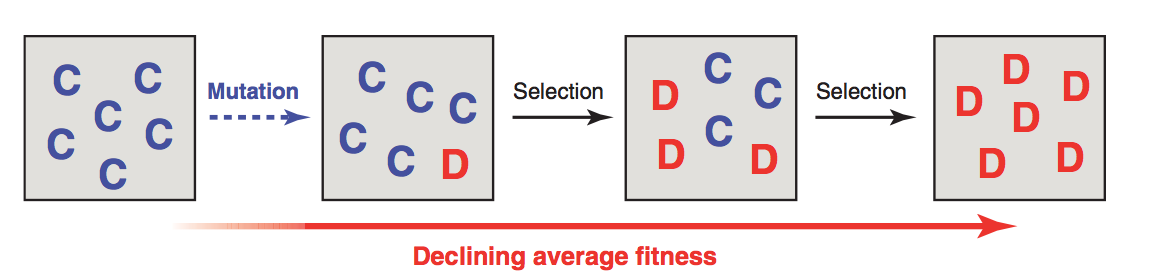
\includegraphics[width=12cm]{figns.png}
  \caption[Natural selection favors defectors]{Natural selection favors defectors \citep{nowak2006five}}
  \label{Figure:figns}
\end{figure}

\subsubsection{Kin Selection}
Kin selection is defined as a rule that cooperative behaviours can have beneficial effect on individuals who have the shared gene. This is reasonable that species carrying similar gene can increase their fitness by cooperation, thus it is supported by natural selection and considered as the consequence of "selfish genes". As it encourages players constantly remain cooperation, it is convinced that the highest fitness will be received. This rule, however, has limitation which is just applied to cooperation between relatives or those have similar strategies.
\subsubsection{Direct Reciprocity}
To explain cooperation between two different species, another mechanism, direct reciprocity, was proposed by \citet{trivers1971evolution} in 1971. He defines it as a new rule for cooperative behaviours between individuals who are not closely related. To be specific, it is assumed that two player can meet again and they can choose cooperation or defection in every round, knowing each other's previous strategy and being able to provide help. Two popular winning solution for playing this game is \textit{tit-for-tat} and \textit{win-stay, lose-shift}. Tit-for-tat is to choose the strategy of what the other has chosen in the previous round which has a satisfactory performance but could not correct mistakes, leading to a continuous retaliation. Win-stay,lose-shift strategy can solve this problem and it is an idea that hold the move when winning and change when you lose. 

If the probability to meet the same players, $w$, is greater than the benefit $b$ to cost $c$ of the altruistic act, direct reciprocity allows evolution of cooperation, as given by \eref{eq:2.3}:
\begin{equation}\label{eq:2.3}
    w > c/b
\end{equation}
\subsubsection{Indirect Reciprocity}
Unselfish behaviours between different individuals in indirect way also can be observed in society. For instance, one person donates to charity but not to direct recipients. In this way, interaction is not symmetric that means it may just has one direction which is different from mutually straight interaction of direct reciprocity (\fref{Figure:figdf}). This type of reciprocity introduces the concept of reputation which is able to be used to form friendship networks. According to \citet{milinski2002reputation}, indirect reciprocity based on reputation can sustain a high level of cooperation, but if there is unexpected indirect reciprocity, fitness will drop rapidly down to zero. On the other hand, reputation can result in higher profits for all players. Although indirect reciprocity is rarely found in nature, it is highly believed helpful to form moral system in human society.

\begin{figure}[!htb]
  \centering
  \subfigure[Direct reciprocity]{
  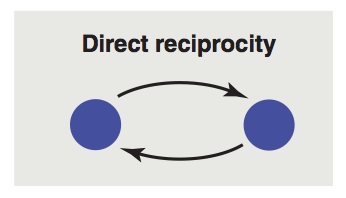
\includegraphics[width=5cm]{dr.png}
  \label{Figure:sfig1}
  }
	\quad
	  \subfigure[Indirect reciprocity]{
	  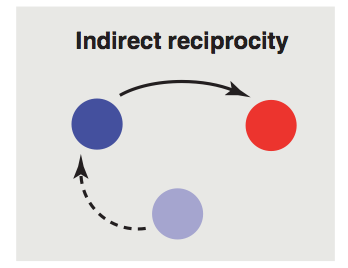
\includegraphics[width=5cm]{indr.png}
	  \label{Fiture:sfig2}
	  }
  \caption[Two mechanisms for evolution of cooperation]{Two mechanisms for evolution of cooperation \citep{nowak2006five}}
  \label{Figure:figdf}
\end{figure}

\subsubsection{Network Reciprocity}
It is common that natural selection is based on unwell-mixed population, where mutual interaction is not equal among individuals. Network reciprocity focus on frequency of interaction of population, assuming populations are not well mixed. \citet{nowak1992evolutionary} argues that without any strategic complexity, forming network clusters where cooperators can assist each other is helpful for cooperators to outcompete.

Network reciprocity can only promote cooperation if the benefit-to-cost ratio exceeds the average number of neighbours, $k$ ,which can be seen as the following equation:
\begin{equation}\label{eq:2.4}
    b/c > k
\end{equation}
\subsubsection{Group Selection}
Group selection is defined as a selection that individuals are formed as a group and suggests that groups with a higher lever of cooperation will defeat those with lower. \citet{traulsen2006evolution} built a model of multilevel selection as follows. A population is subdivided into groups where cooperators help each other but defectors do not. Members of a group determine their strategy based on fitness in an evolutionary game. Gradually, offspring are added to the same group, resulting in enlargement of individuals with similar strategy. If a group reaches a certain size, it will split into two. Division continues in those groups with faster reproduction. Then competition between groups emerge because of different speed of group growth. In particular, defection happens more within a group than collective behaviours does, whereas pure cooperator groups grow faster than pure defector groups. That means selection is different in multiple levels - on the lower level, it is more likely to defect, but on the higher level selection favours cooperators.

Mathematically, in order to favour cooperation, the relation between the benefit-to-cost proportion and the ratio of the maximum group size $n$ to number of groups $m$ should satisfy the condition as follows:
\begin{equation}\label{eq:2.5}
    b/c > 1+ (n/m)
\end{equation}
\subsection{Spatial Prisoner's Dilemma Game}
Prisoner's dilemma game, which was clearly introduced in the previous section, has been studied to look for optimal strategy for conflict between selfish individuals and altruistic behaviour. Generally, spatial prisoner's game is assumed that an individual can interact with four immediate neighbours, deciding either cooperation or defection.Total payoff depends on each two players' strategy combination in which has been defined in the so-called payoff matrix. Recent research has concentrated on modelling spatial prisoner's dilemma game.

 \citet{nowak1992evolutionary} introduces a two-dimensional spatial game as follows. Prisoner's dilemma is applied as a basic fitness matrix, only considering two strategies - cooperation and defection. Every player plays against the nearest neighbours in each round and the winner who receives the highest payoff will occupy the site. Afterwards, a second round starts as the previous rules and it may iterate for finite times. Without remembering players or strategies, this model can generate a spatial pattern that contains indefinite collective and treacherous behaviours. Eventually, it is found that introduction of spatial structure can promote formation and maintainance of cooperative clusters to resist invasion from defectors. Interestingly, they found sequence of evolutionary spatial prisoner's dilemma game can be extremely beautiful which can be seen in \fref{Figure:wanhuatong}.
 \begin{figure}[!htb]
  \centering
  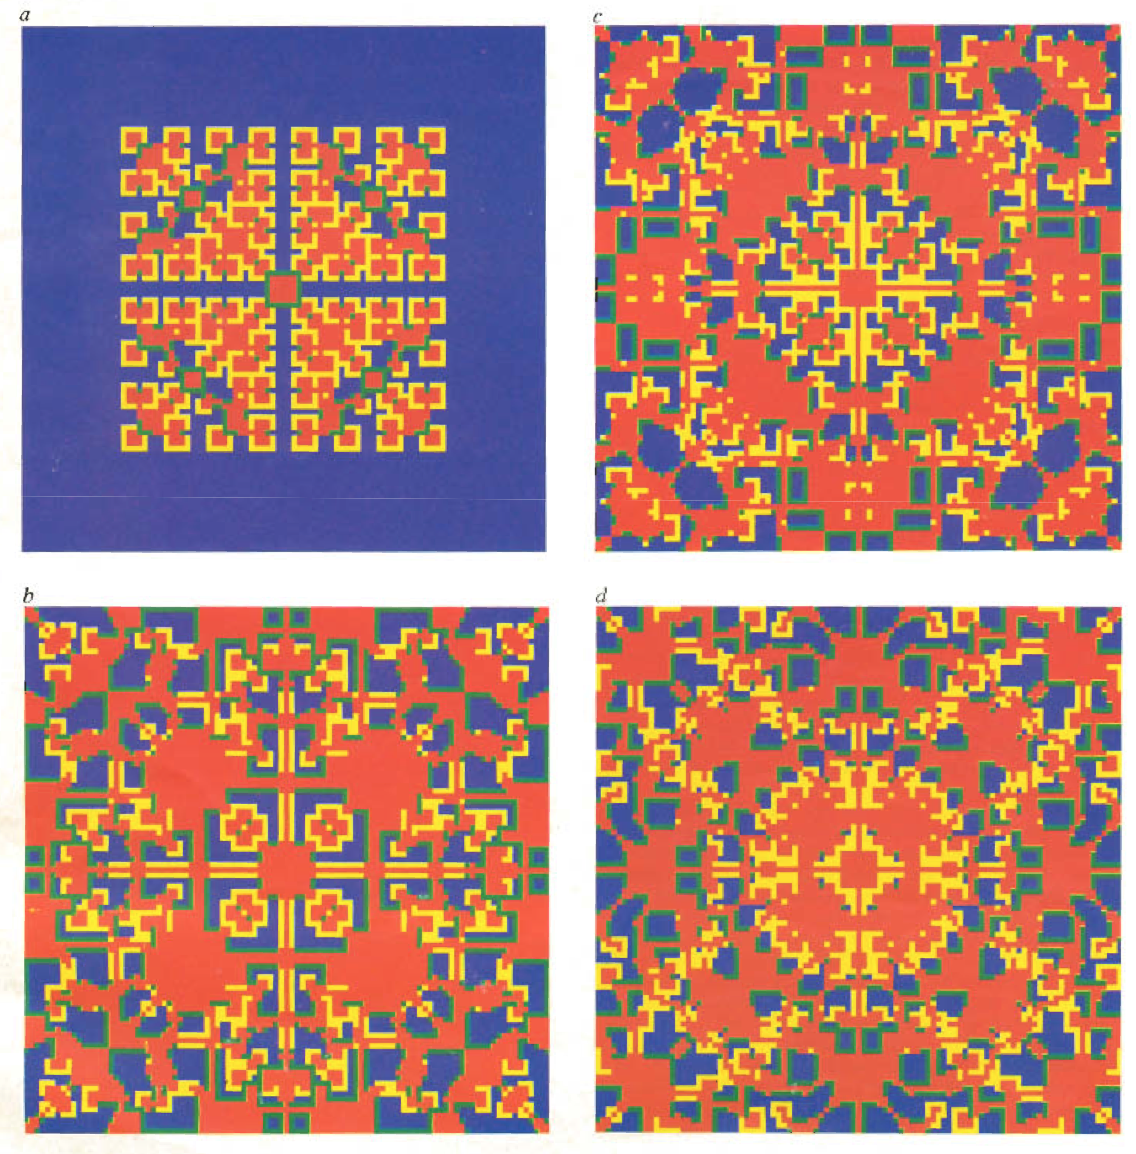
\includegraphics[width=8cm]{wanhuatong.png}
  \caption[Evolutionary kaleidoscope generated by spatial games]{Evolutionary kaleidoscope generated by spatial games \citep{nowak1992evolutionary}. Blue represents cooperation which cooperated in the previous game and red is defection following the same strategy. Yellow is defection following cooperation, while green describes cooperation following defection.}
  \label{Figure:wanhuatong}
\end{figure}

In addition, there are some other models relating to prisoner's dilemma game on a square lattice. A new model is created by \citet{szabo1998evolutionary}. Specifically, the fitness matrix is created as  \citet{nowak1993spatial} suggest, "reward" R=1, "punishment" P=0, "sucker's payoff" S=0 and "temptation" T=b where $b>1$. Therefore, what a defector can get most is $4b$ whereas a cooperator can receive 5 totally if the surroundings are all cooperators. In this model, a randomly picked player has a probability to adopt the neighbour's strategy which can be shown as \eref{eq:2.6}
\begin{equation}\label{eq:2.6}
   W=\frac{1}{1+exp[-(E_Y-E_X)/K]}
\end{equation}
where $E_X$ and $E_Y$ denote total payoffs of player X and Y, respectively and $K$ is the noise allowing irrational decisions. This game will be played for finite time.

\section{Migration Games}
\subsection{Neighbourhood structure}
\subsubsection{Static Neighbourhoods}
Static neighbourhood structure assumes all players are categarised in different groups and individuals in the same group will not change to another group. For example, players who play a specific video games, especially multiplayer online battle arena, can be divided into a grandmaster, a national master, a professional or an amateur. Generally, grandmasters play among themselves, professional players play with those professional and so on. Professional people will upgrade to grandmasters or degrade to an amateur. According to \citet{lecturePPT}, there is a theorem: \textit{let G be a neighbourhood graph and let m be the number of neighbourhoods (cliques) and let M be the maximum size of a clique. If all the players are of the same type t then the game stabilises in at most $mM$ steps.} In this theorem, type $t$ can be defined as follows: if the payoff in round $K$ is greater than 0.5, then play with the same action. If all players use a different strategy, then change to this strategy in the next round. In this case, it is similar to the "win-stay, lose-shift" solution.
\subsubsection{Dynamic Neighbourhoods}
Dynamic neighbourhood structure allows players move between groups. In the model given by \citet{lecturePPT}, players change to the neighbour's group when the neighbour's payoff is greater than his, otherwise stay the same. To make the population stable, it should take $n^{n(n+1)/2}$ steps at most.

To make the definition of dynamic neighbourhoods clearer, an example can be described like a vegetable seller with pushcarts in the market \citep{paul2011neighbourhood}. First of all, the location can dynamically changed according to the demand of this neighbourhood, who sells around and how well other sellers do. Moreover, product is flexible based on different preferences in the neighbourhood and determined by a complex rationale. Finally, the price varies depending on general market situation. If selling in a poor community, the price should be affordable for citizens there. In this instance, location modification can be thought as change between groups and others represent the player's strategy which can be determined in many aspects by how much payoff can be received.
\subsection{Experiments on Migration Games}
In the paper of \citet{helbing2009outbreak}, success-driven migration is proposed that it can promote cooperation in a spatial game. In prisoner's dilemma game, clusters of cooperators can get the most payoff which means if all cooperators stay together without defectors, fitness will maximise. Therefore, in Helbing and Yu's model, cooperators leave the neighbourhood which contains a defector and look for more favorable ones and remain in cooperative neighbourhood. In this case, it satisfies with ESS which can form cooperative population and it is immune to defection.











\chapter{Design}
A web-based game needs effective interaction with users when they are playing the game, which is thought to be very essential in this user-oriented era. For example, Windows operating system is in some case considered less user-friendly than Mac OS X partly because it lacks of detailed responsive mechanisms for user operation, especially when an application is running backstage. For example, when a software is loading slowly, Windows just shows users a pointer, representing it is running which is occasionally  misunderstood as system halt. Instead, Mac makes the icon bouncing to tell users it is running, even though it is very slow. In a word, interaction is important for programming. Back to the project, ensuring response to every individual's operation in time and tell them what they should do next as a guidance is one fundamental principle. To achieve this, the web page should have an accessible user interface and efficient data structure. In terms of logic, there should be a policy that administrators can control or configure the game, including agreeing or disagreeing users to access and deleting an account from the user list. It is of importance that users can smoothly play the game as well. In this section, how to design in three aspects will be introduced.
\section{Overall Design}
In general, the basic architecture can be divided into three blocks - \textit{user} which consists of player and administrator, \textit{web server} and \textit{database}, as illustrated in \fref{Figure:fig33}. Players are able to play the game, but they cannot join until an administrator approves. Data should be validated before it was saved which occurs in the client side. Moreover, users operations, which cover all the operations of users in this project, should response immediately, so they are executed on the web browser. Administrators are responsible for managing the whole system, replying for users' requests and monitoring users. All of their actions will be sent to web server where requests are handled. For example, when jumping to another page, a request is sent to server and after processed, server will returns the feedback. In addition, requests of data storage should be executed on server side. When data operation is needed, data will be sent to the server and handled by the server, then sent to database. Database, as normal, is a disk for storing data in order to have an analysis in the future. These three modules coordinate and communicate with each other and have different responsibilities - operation by users, event handling by the server and information saving by database.

\begin{figure}[!htb]
  \centering
  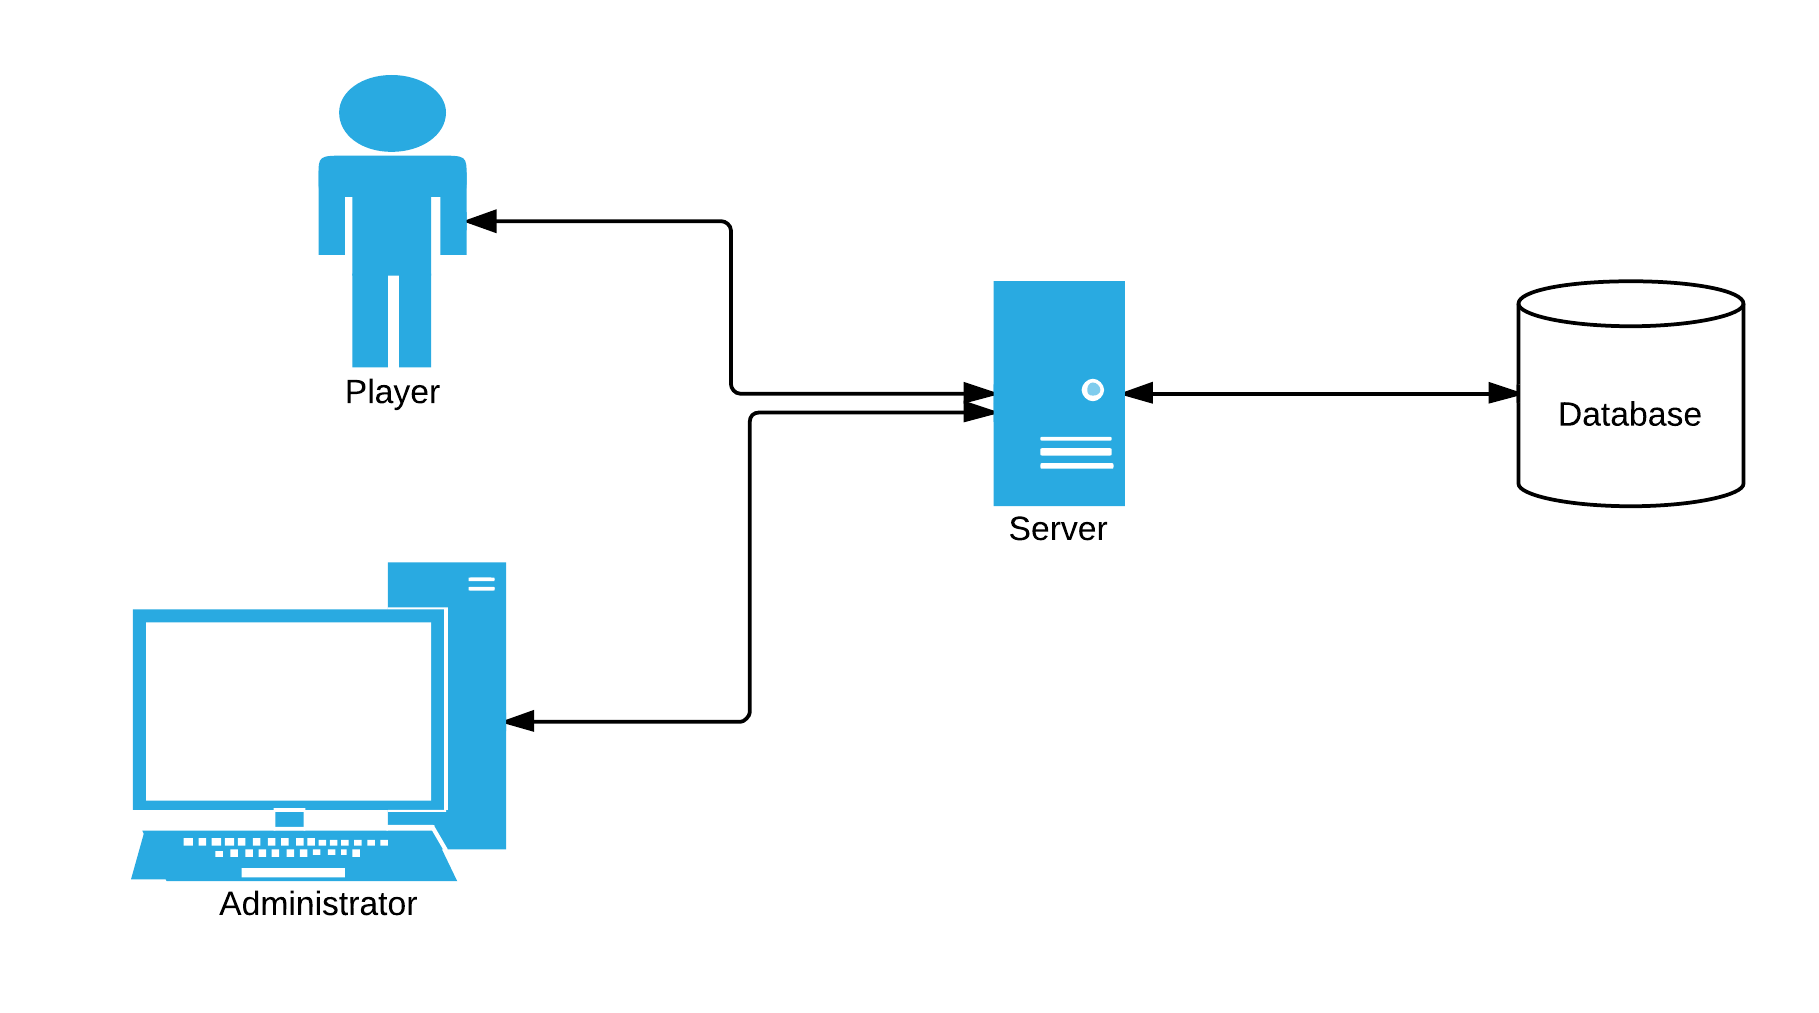
\includegraphics[width=10cm]{model.png}
  \caption{Application architecture}
  \label{Figure:fig33}
\end{figure}

\section{User Interface}
User interface is an integrated layer offering communication and logic operations between clients and machines. It is the surface of an application which can leave a good expression for users. User-friendly, comfort and easily used are its principles which could provide users convenience and efficient interaction with computers.



\subsection{Administrator}
As can be seen in \fref{Figure:fig35}, logging on to the administrator window, there should be a drop-down list to choose among showing all users, users on request and users who have been approved to participate in the game. By picking up different choices, relevant tables should be shown below the drop-down list, containing various operations the administrator can do. For example, in the user-on-request table, deletion and agreement can be executed and they should be implemented as buttons after every record. When clicking on the button, action will be activated and executed.
\begin{figure}[!htb]
  \centering
  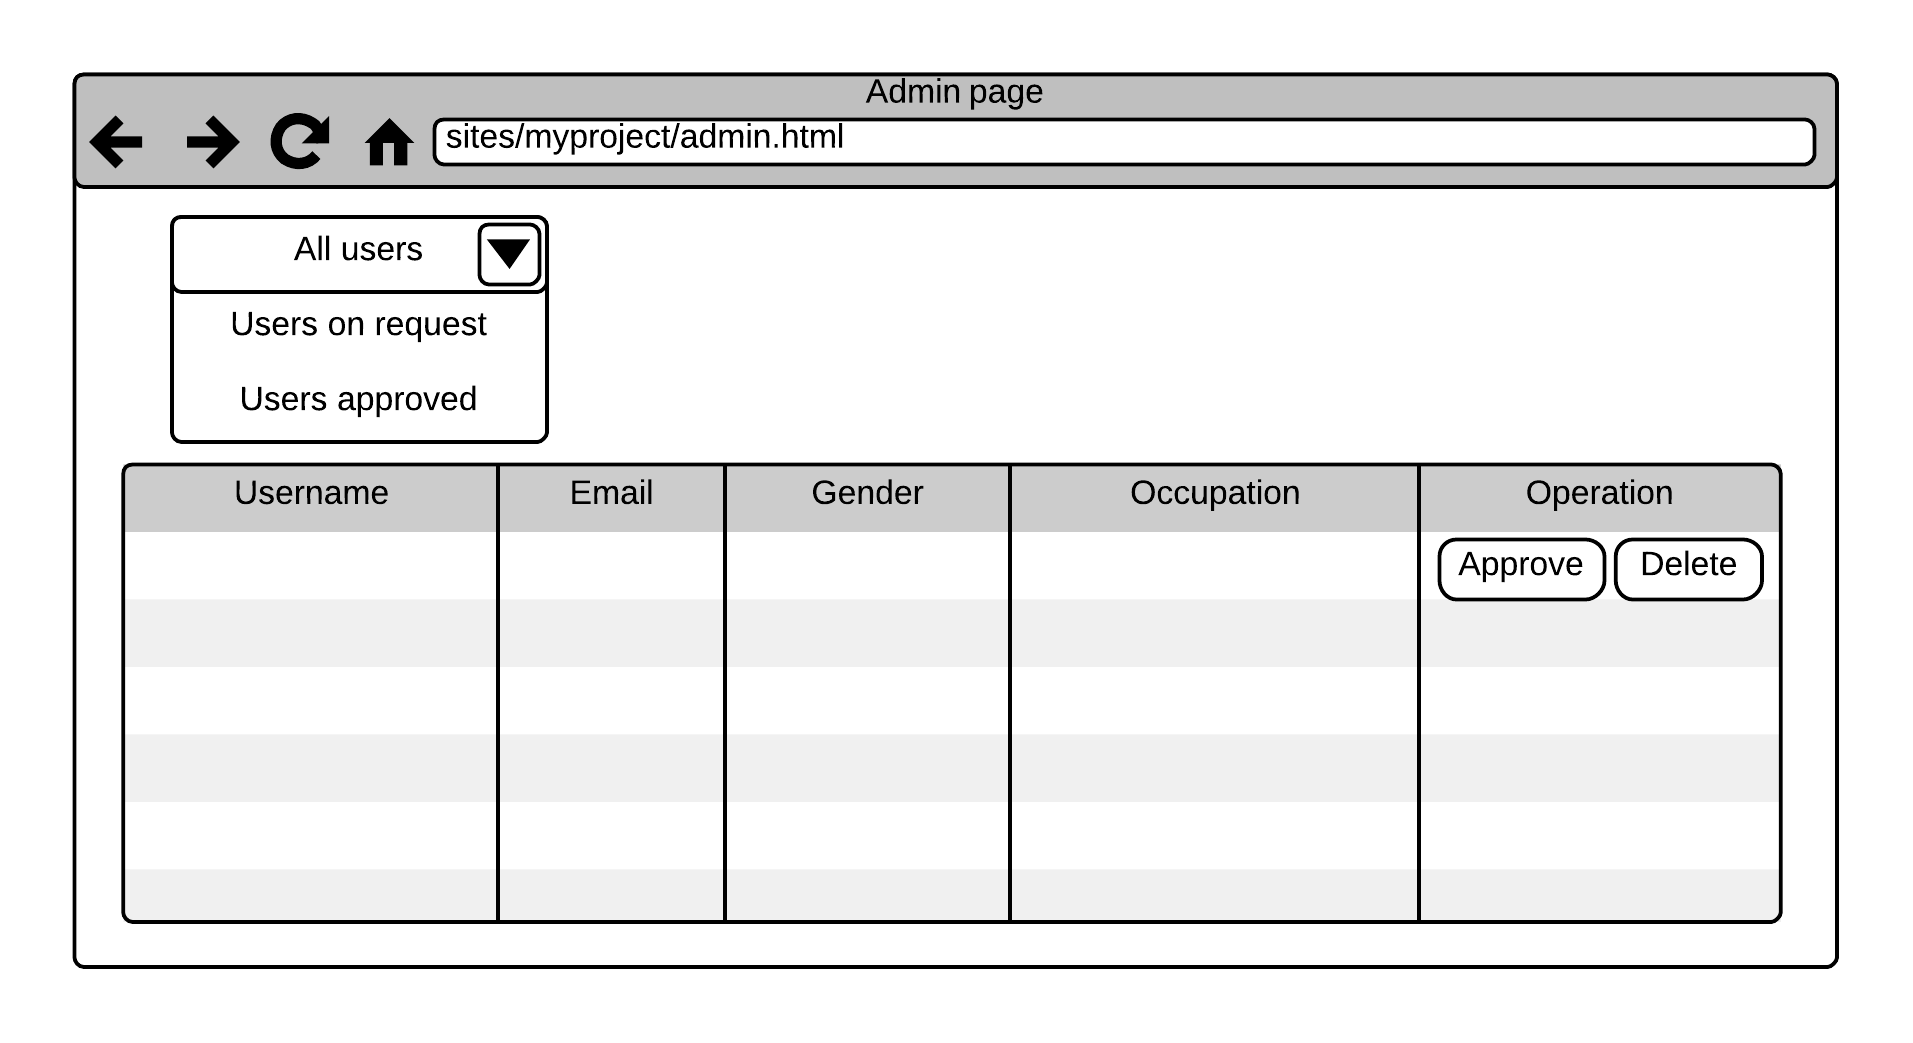
\includegraphics[width=11cm]{admin_page.png}
  \caption{Administrator page}
  \label{Figure:fig35}
\end{figure}

\subsection{Normal User}
Normal users will have two key components - \textit{instruction page and main game page}. On the instruction page, content is concise and paragraphs are separated clearly. In addition, font size should be as big as 12 point typeface which can be probably distinct enough to read. For the registering part, personal detail such as username, email and occupation should be entered in text boxes, while gender could be chosen between "Male" and "Female" and it can be achieved as a "radio" label.

Furthermore, log-on page is simple that it has two text boxes for username and password and a button to log on. When the main game page is opened, it should be roughly split into four parts, as shown in \fref{Figure:fig34}. On the left top side, it is an information module, which shows messages regarding to guidance of the game. It displays the result of last round and teaches what the player should do in the next step. Below the information module, there is an icon instruction, showing meanings of diverse icons in the map. Moreover, the prisoner's dilemma matrix will be placed in it. The main map is in the middle of the whole page, which will design as a chessboard, a 10$\times$10 table. On the chessboard, black point represents defector while white point is cooperator whose colours are contrast to each other and it could offer players clear distinction of cooperators and defectors. Furthermore, an image of  a person is on behalf the location of the player all the time. The last icon on the living area is question mark and it is the occupied location but the actual strategy is unknown which will be discovered when a player migrates to be a neighbour.All the operating buttons are on the right hand side, including cooperation, defection and other control buttons. As a whole, the core of the game is in the middle which can let users focus on the game and its left side is description while the right hand side is the operation module.

\begin{figure}[!htb]
  \centering
  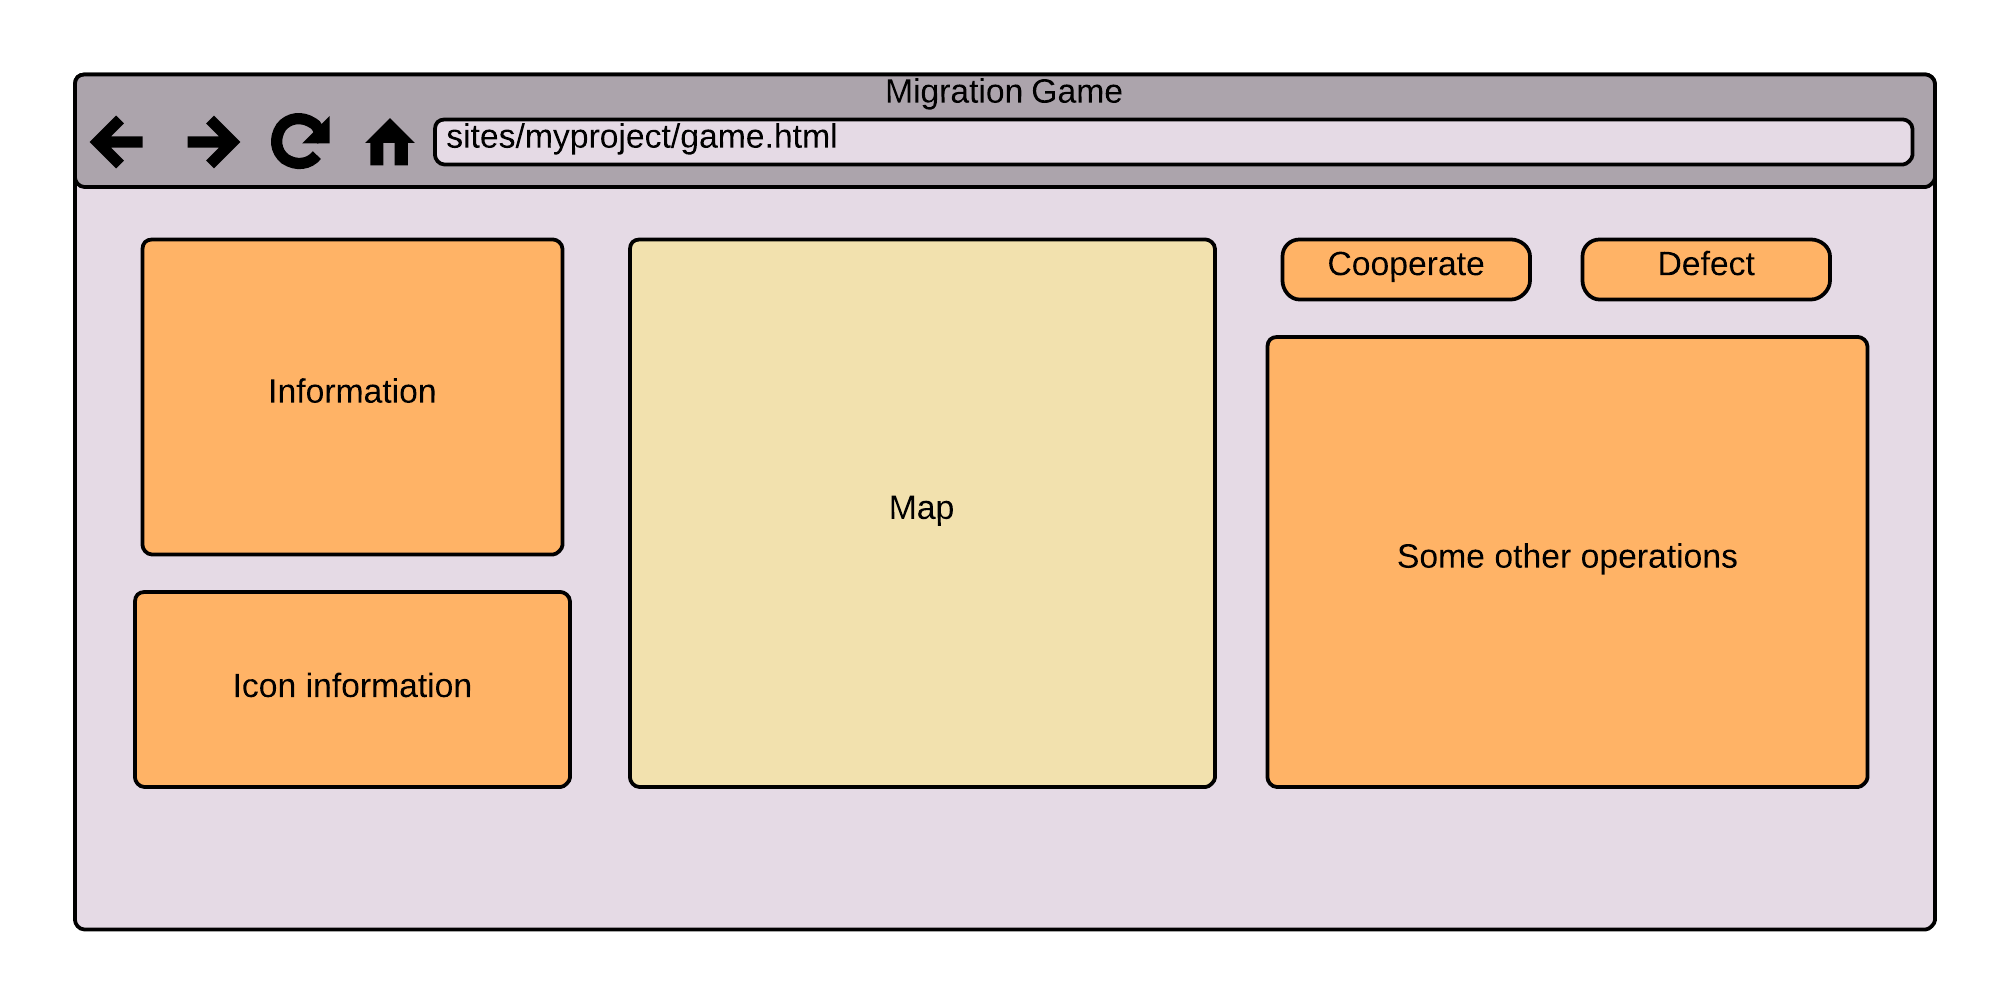
\includegraphics[width=14cm]{game_page.png}
  \caption{Game page}
  \label{Figure:fig34}
\end{figure}



\section{Business Logic Layer}

Business logic which is the core of application architecture is the connection between user interface and data access layer. A reasonable logic design is always beneficial to future maintain and extend. To be specific in the project, game procedure comes first before continuing to develop. \fref{Figure:fig32} shows the whole prcess from a user opening the webpage to storing record in the database and \fref{Figure:fig31} describes the detailed game procedure. As a whole, the procedure can be listed as follow:

\begin{figure}[!htb]
  \centering
  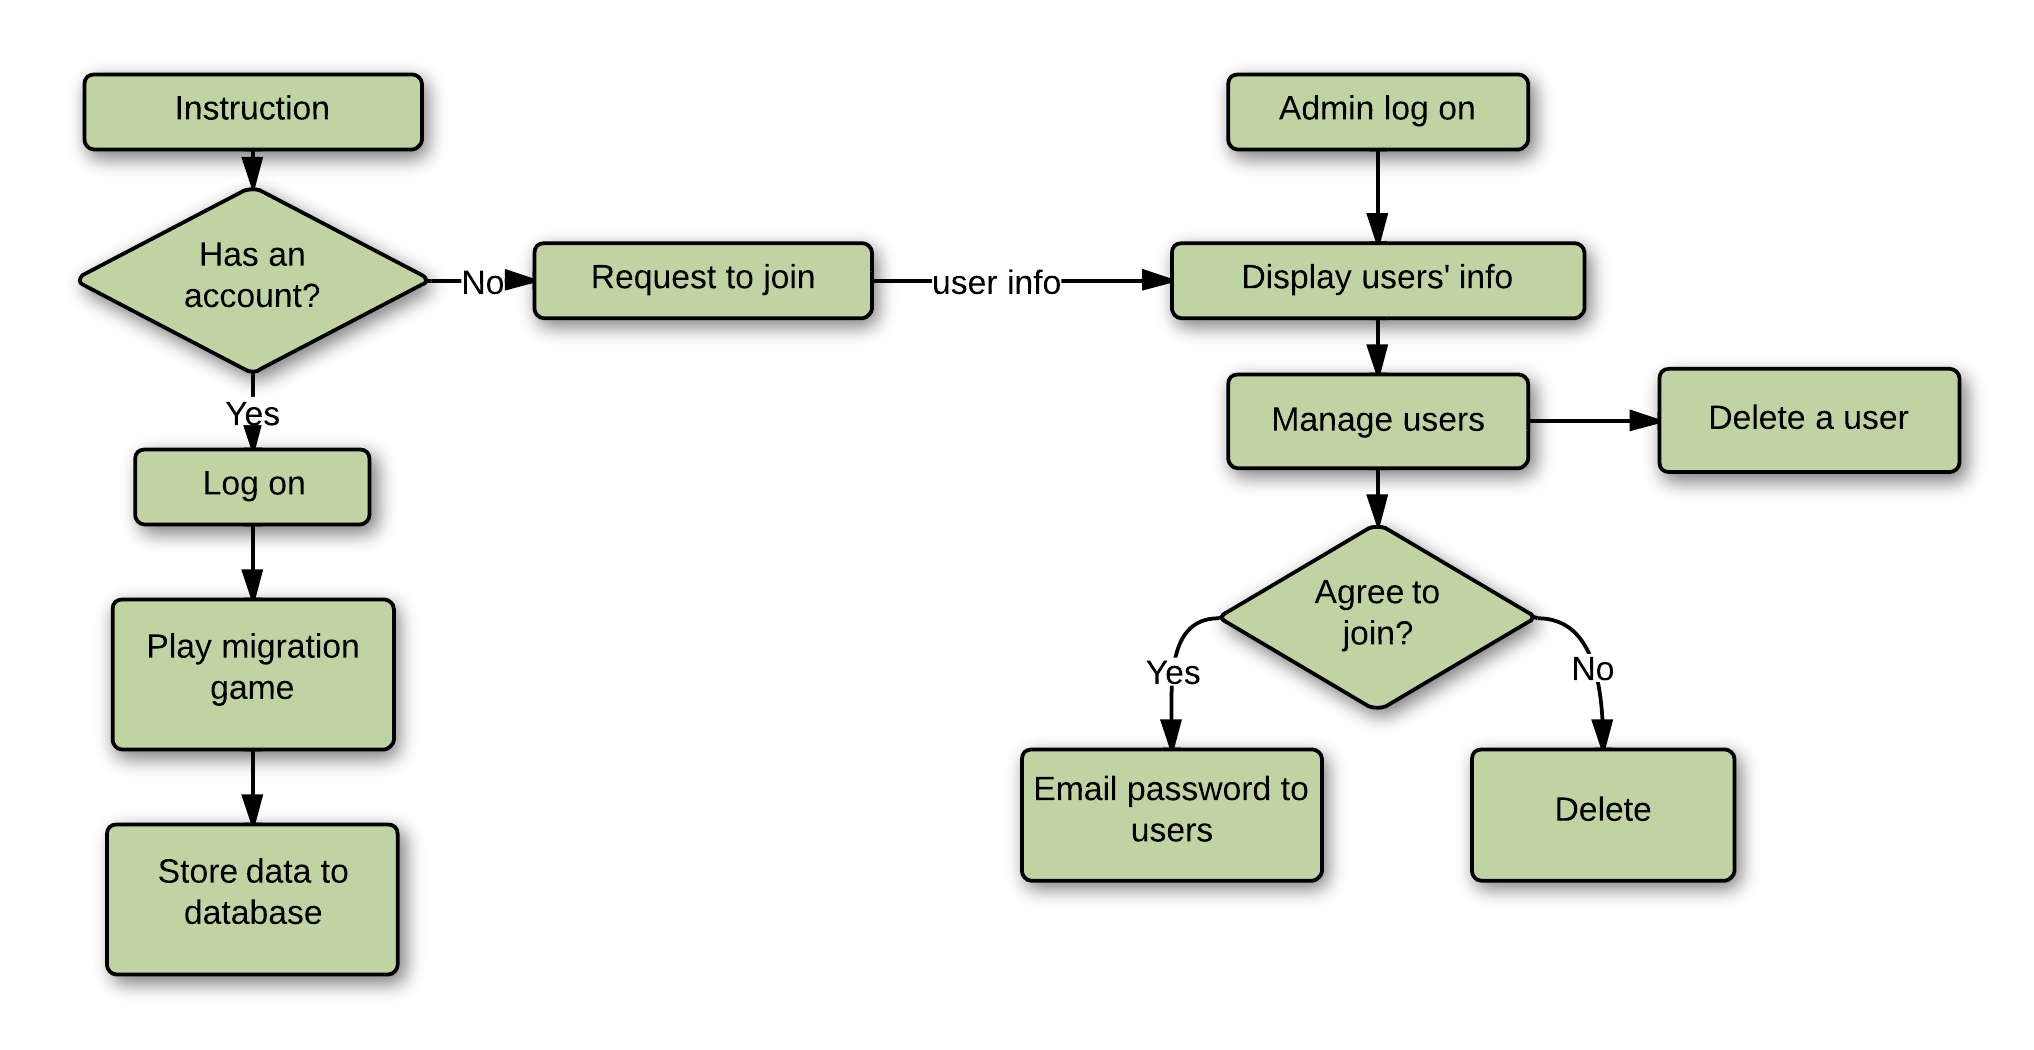
\includegraphics[width=12cm]{procedure.png}
  \caption{The whole process}
  \label{Figure:fig32}
\end{figure}

\begin{figure}[!htb]
  \centering
  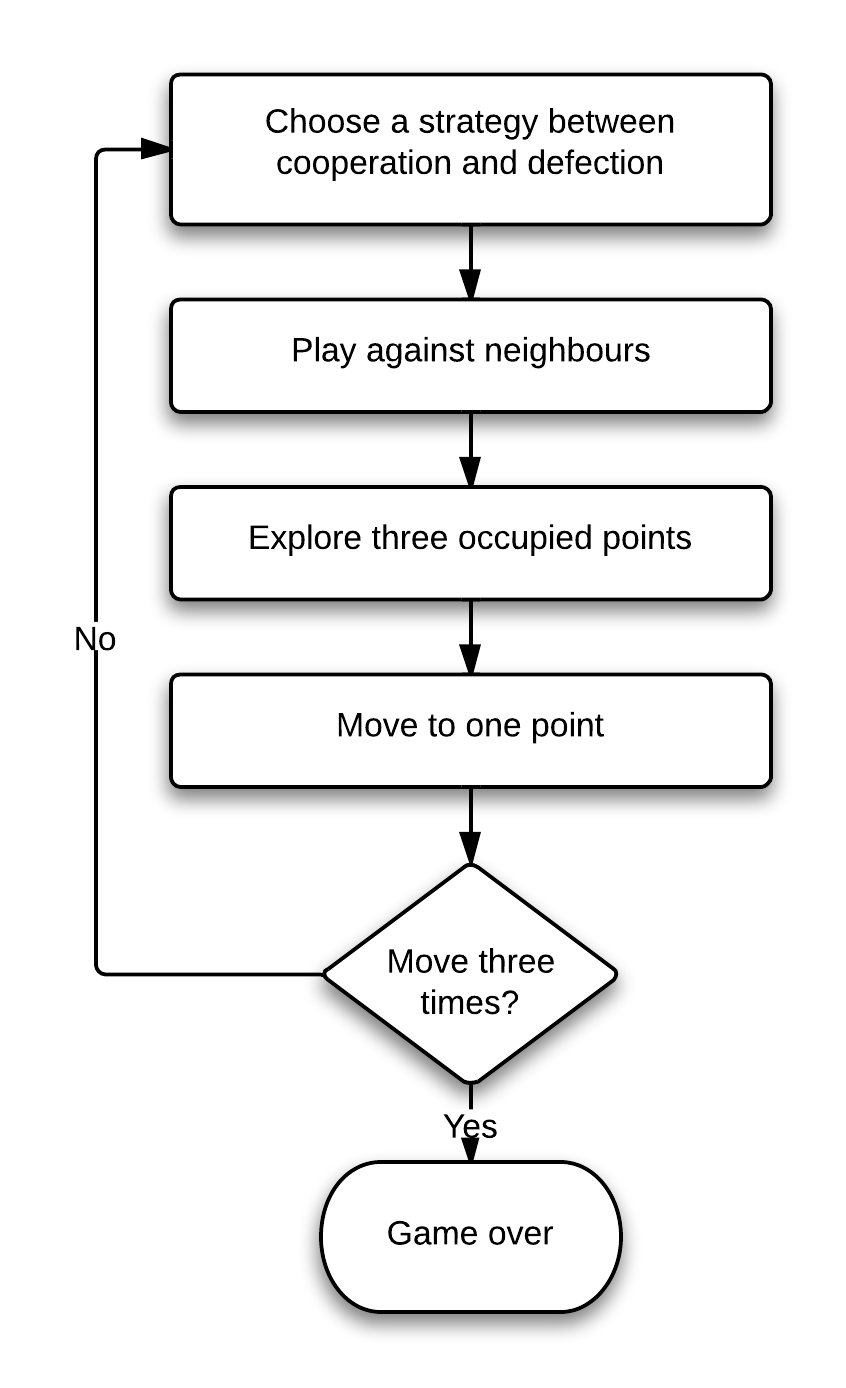
\includegraphics[width=6cm]{flow.png}
  \caption{Migration game procedure}
  \label{Figure:fig31}
\end{figure}

\begin{enumerate}
\item A user reads through the instruction of migration game and registers using his or her email address. In addition, a few personal detail should be sent as considering factors for administrators.
\item The administrator visits the managing page to monitor all the users. If a user is allowed to join the game, an email with a random password would be sent to the user which can be used to log in the game.
\item When a player enters the game, a randomised map is shown representing the living area, involving the player's initial position, occupied places whose strategies are unknown and some empty points. 
\item The player can choose the first strategy to play against his or her four neighbours and get corresponding payoff based on different combination of neighbours' strategy. The payoff matrix "abides by" prisoner's dilemma.
\item Three empty points can be explored by the player which will return corresponding bonus at this point and mark on it.
\item Move to one empty point according to exploration.
\item Users can choose strategy again and use it to play with neighbours. Then a feedback of payoff will be displayed and tell the player to continue to explore.
\item It will repeat for three times and user will get the final payoff at the end of the game.
\item All the data will be sent and stored in the database which can be visited by the administrator.
\end{enumerate}
When process is determined, how every component can be achieved should be designed next. First of all, for the instruction and register component, it is the entrance of the whole game which is able to leave a good impression for users and offer them necessary information to join the game. Detailed explanation is presented teaching people how to play the game, including what every symbol stands for. Moreover, content that the player types in should be validated before sending to the server which is definitely efficient and more secure. For example, username, email address and occupation cannot be empty and email address should be in the email format, thus the data of email can be all in same format and guarantee successful confirmation of a user's authority by email. If information is entered wrong, there will be a warning telling users to enter again. After sending the request, the user will receive a note asking to wait for the approvement. 

By clicking into the log-in page and logging on with username and password which is randomly generated, the main game will be displayed which should be split into three parts - \textit{guidance, operation and chessboard}. The guidance is responsible for showing results of the user's last action and details of what a user should do in the next step. Users play the game by hitting buttons on operation part  which will change according to the game procedure for clearly showing on which move the player is and how they can continue to play. The core of the game, chessboard, should be a 10$\times$10 table presenting the living block a person is and all manipulations directly affect and reflex on this map. In the game flow, people can choose an occupied place to explore and an empty location to move, so the map should be able to click and return some click events, such as displaying the corresponding bonus and revealing the actual strategy in a specific location. Also, each time a person move to a new place, all the neighbours should be known and payoff is automatically calculated, then how much he or she could acquire if migrating to here should be described for the user.

\section{Data Access Layer}
\begin{figure}[!htb]
	\centering
	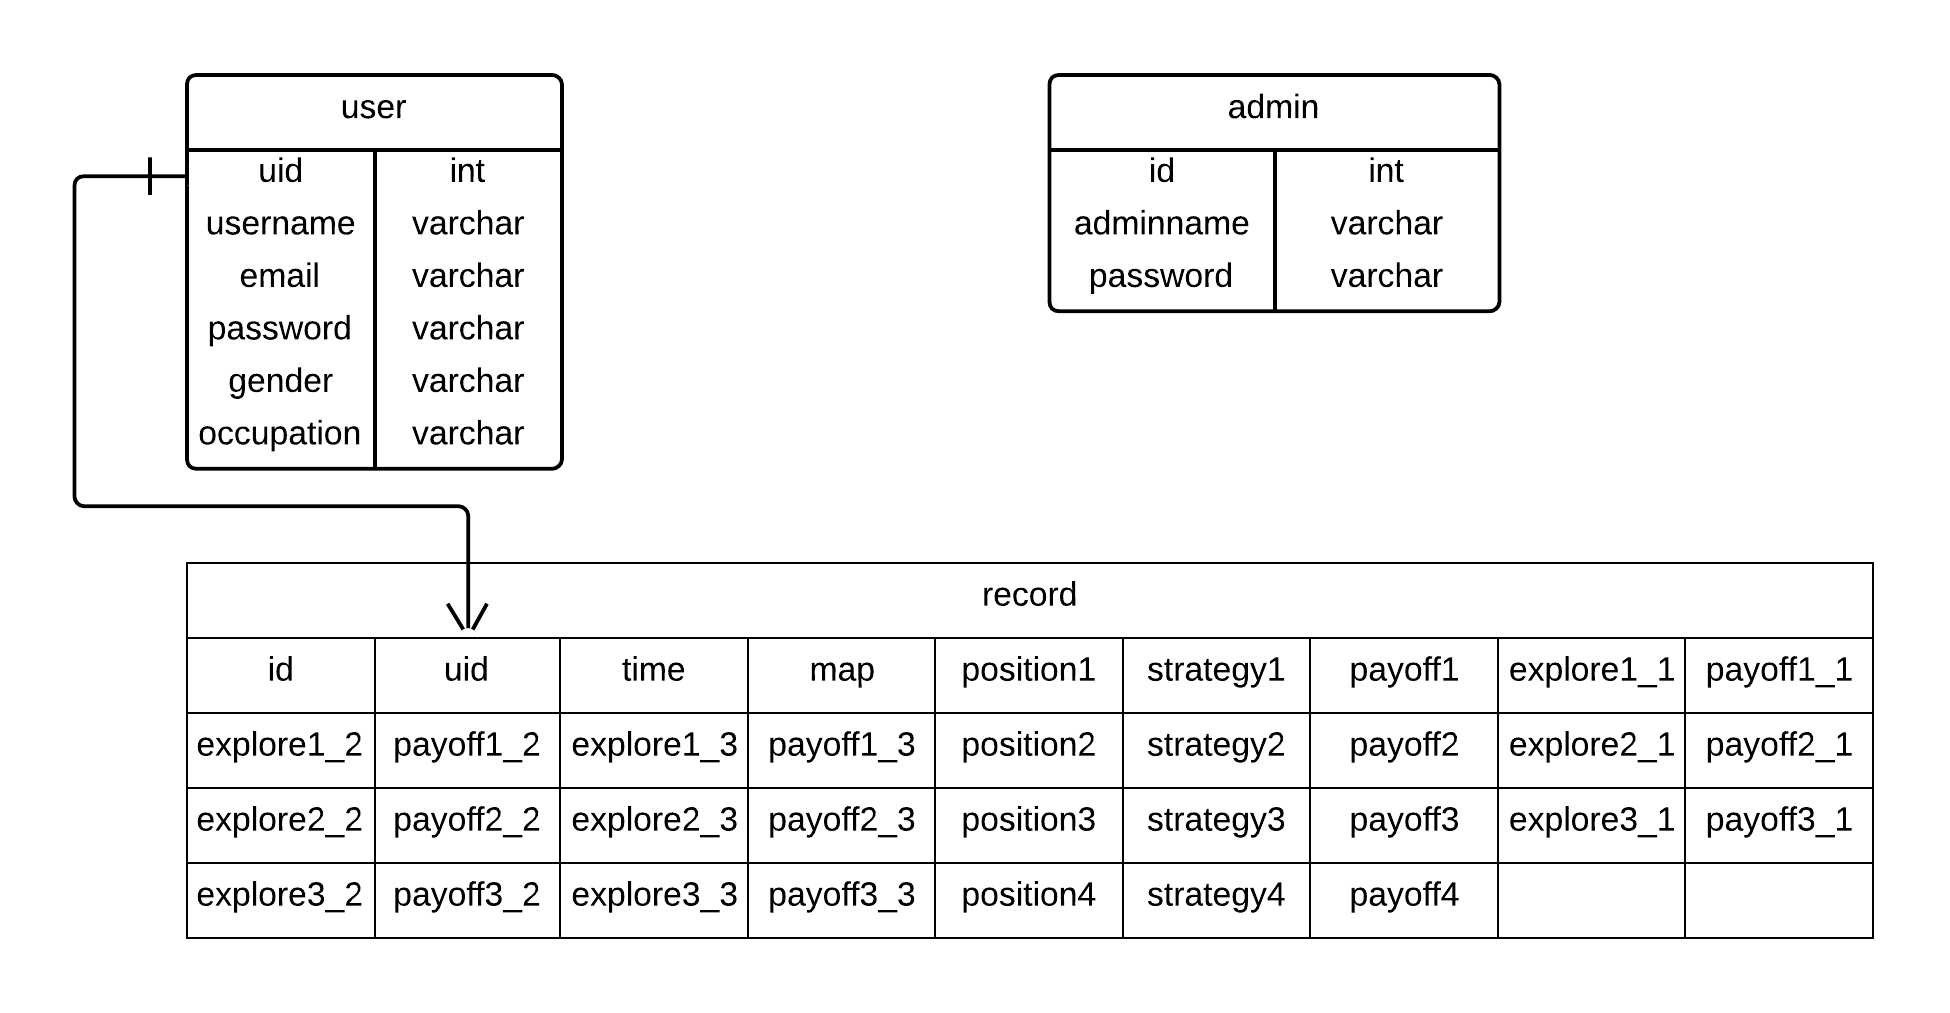
\includegraphics[width=14cm]{database.png}
	\caption{Database diagram}
	\label{Figure:figdb}
\end{figure}
The function of data access layer is to control the data flow in the database, including selecting, inserting, updating, deleting. In this project, all data is used "post" method to deliver values from html to php which is more secure. As \fref{Figure:figdb} shows, it contains three tables - \textit{user, administrator and record}.

 "Admin" has id of an administrator, name and password. When an administrator wants to log on, a select query will be executed and return the corresponding id value. If the system needs to add a new administrator, it should be directly inserted in the database which may be relatively inconvenient but more secure. 
 
The "user" table has user id, user name, email, password, gender and occupation. When a new user registers, a new record would be inserted except the password which cannot be added until the user is approved by the administrator. When he or she is agreed, a 9-digit password will be randomly generated and update the password in "md5" format which means it is encrypted and no one can read it even administrators. "State" of a user describes what status he or she is. For instance, "0" means this user has not been agreed while "1" represents the opposite meaning. In addition, user log-on action will activate a select query to test if the typed username and password exist. If the user exists, it will return the id value. Otherwise, "null" will be sent back.

The most complicated table is the "record" which stores all the data of the game. To be specific, every game has an id and who and when plays this game. Because the map is randomly initialised at the beginning of the game, it can be saved as an array. Position 1 to 4 are the player's locations every time. Similarly, strategy and payoff each round can be saved (strategy 1 to 4 and payoff 1 to 4 respectively). Additionally, coordinates of exploration and payoff at each searching point are recorded that it should be definitely necessary for the future analysis of human strategy. All these information is only inserted at the end of the game and just can be accessed by the administrator.







\chapter{Implementation}
The project is programmed through HTML, CSS, JavaScript, PHP and MySQL. HTML, CSS and JavaScript are responsible for the front end which includes presentation of web page and every click event handling. The back end data is processed by PHP which actually interacts with database. In this chapter, how every key functionary is achieved by code will described.
\section{Instruction Page}
Instruction page provides information about the migration game and it is also a registering entrance. In general, this page is implemented by HTML and PHP. Paragraphs are clear with 18 pixel font size, informing what users can do during the game. Registering part has connection with database, inserting user information . All typed content would be validated by testing whether they are empty (Listing 4.1). Whichever is empty, an alert window will pop up and the cursor will focus on where is empty.
%\begin{figure}[!htb]
	%\centering
	%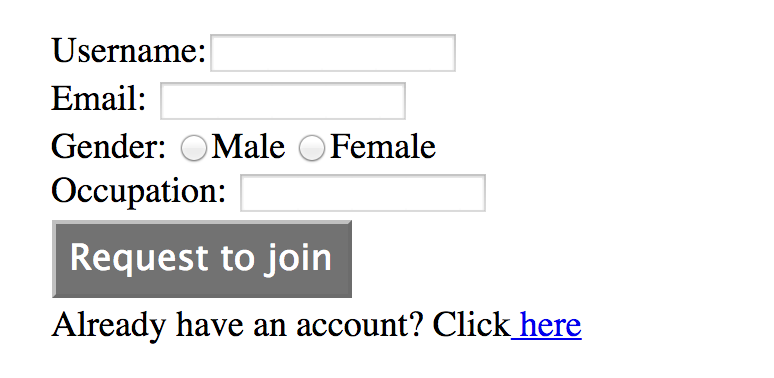
\includegraphics[width=8cm]{register}
	%\caption{Register segment}
	%\label{Figure:figRgst}
%\end{figure}

\begin{lstlisting}[caption=User data validation segment]
function inputCheck(registerForm){
	if(registerForm.username.value==""){
		alert("Please enter your username.");
		registerForm.username.focus();
		return(false);
	}
	if(registerForm.email.value==""){
		alert("Please enter your email.");
		registerForm.email.focus();
		return(false);
	}
	if(registerForm.occupation.value==""){
		alert("Please enter your occupation.")
		registerForm.occupation.focus();
		return(false);
	}
}

\end{lstlisting}
Eventually, the instruction page is implemented like \fref{Figure:intro}. Instruction of this game is described from the top and at the bottom of this page, there is a registering component. A style of "hover" is added in the button, so that when the mouse moves upon the button, the colour will be changed.
\begin{figure}[!htb]
  \centering
  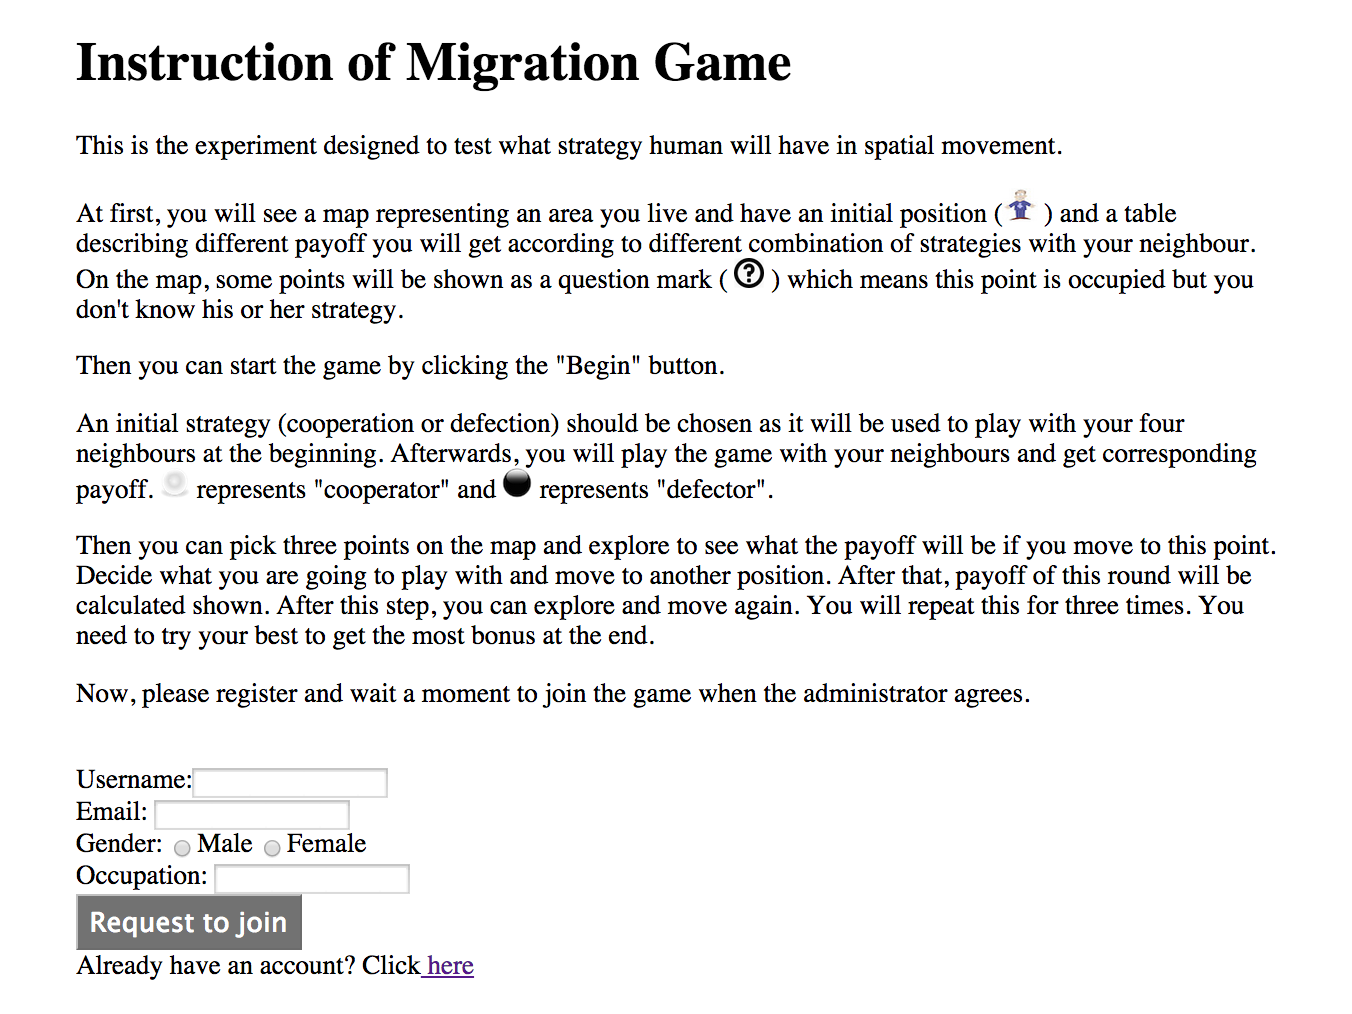
\includegraphics[width=14cm]{instruction.png}
  \caption{Intstruction page}
  \label{Figure:intro}
\end{figure}


\section{Log On Page}
The log on page of users is similar to that of administrators which has two labels of an administrator's name and the password, enclosed by a $\langle legend \rangle$ element. Every time a manager logs in, a SQL query like \textit{"SELECT id FROM admin WHERE adminname='\$adminname' AND password='\$password'" }will be executed. If it fails, the person can try again.

\section{Administrator Page}
\subsection{User List}
To make the page more efficient, "Ajax" is used in order not to refresh the whole page every time an option is selected. The source code is presented in Listing 4.2 which is called when the value of the $\langle select \rangle$ element that includes values of "all users", "users on request" and "users agreed" is changed. Relevant records in the "user" table will be chosen and displayed as a table which is completed in a php file - "getuser.php". In the "getuser.php" file, a specific table is exhibited by selecting users according to the "state" value and using "echo" to output.

\begin{lstlisting}[caption=Ajax segment for listing users]
function showUser(str){
		if (str=="") {
    		document.getElementById("txtHint").innerHTML="";
  		  	return;
  		} 
  		if (window.XMLHttpRequest) {
    		// code for IE7+, Firefox, Chrome, Opera, Safari
    		xmlhttp=new XMLHttpRequest();
  		} else { // code for IE6, IE5
    		xmlhttp=new ActiveXObject("Microsoft.XMLHTTP");
  		}
  		xmlhttp.onreadystatechange=function() {
    		if (xmlhttp.readyState==4 && xmlhttp.status==200) {
      			document.getElementById("txtHint").innerHTML=xmlhttp.responseText;
    		}
  		}
  		xmlhttp.open("GET","getuser.php?q="+str,true);
  		xmlhttp.send();
	}

\end{lstlisting}

\subsection{User Management}
Administrators have the right to control the game or the application, therefore some operations against users should be accomplished. In this project, an manager can administrate users by deleting and approving.

If a user is disagreed to take part in the game, he or she could be deleted. In the listed table of players, deletion is one of the two activities for each individual. When this button is clicked, a new URL will be generated by adding the user id value which would be deleted at the end and direct to another php file which interacts with the real database. A "delete" query will be activated which should be \textit{"DELETE FROM user WHERE uid='\$uid'"}. The "uid" value can be obtained through URL.

A password can be sent to a user by email by the "email" button is clicked. There are two key problems to be solve. How to pass the value of who needs to agree is the first question and the solution is pass necessary values through URL. When a user is approved, the user id will be put at the end of the url, thus the php can know whose email is going to be sent to and then execute it. In addition, two package are imported for email sending which are "class.phpmailer.php" and "class.smtp.php". They are open source in the Internet and specify to securely send an email by SMTP. As shown in Listing 4.3, both of them are required and then it configures some fundamental variables such as host address, SMTP username and password. After email sent, the 9-digit randomly generated password will be encrypted by MD5 and saved in the "user" table and update state of the user into "1" which means having been agreed.
\begin{lstlisting}[caption=Email segment]
require ('class.phpmailer.php');
require ('class.smtp.php');

$mail = new PHPMailer;
$mail->isSMTP();                                      // Set mailer to use SMTP
$mail->Host = 'smtp.gmail.com';  // Specify main and backup SMTP servers
$mail->Port = 465;
$mail->SMTPAuth = true;                      // Enable SMTP authentication
$mail->Username = '$my email address';                 // SMTP username
$mail->Password = '$my email password';                  // SMTP password
$mail->SMTPSecure = 'ssl';                // Enable encryption

$mail->From = 'kevininsoton@gmail.com';
$mail->FromName = 'admin';
$mail->addAddress($email);     // Add a recipient

$mail->addReplyTo('huntingkevin89@gmail.com');
$mail->WordWrap = 50;

$mail->IsHTML(true);    // set email format to HTML
$mail->Subject = "Migration game password";
$mail->Body = "Welcome to migration game! Your password is ".$password.". Please use it to log in the game.";

\end{lstlisting}

The administrator's page is displayed in \fref{Figure:admin} which contains a drop-down list choosing among different users' types - on request and agree. The result is listed below, with some information of every user. The administrator can delete which means reject here, and email or approve.
\begin{figure}[!htb]
  \centering
  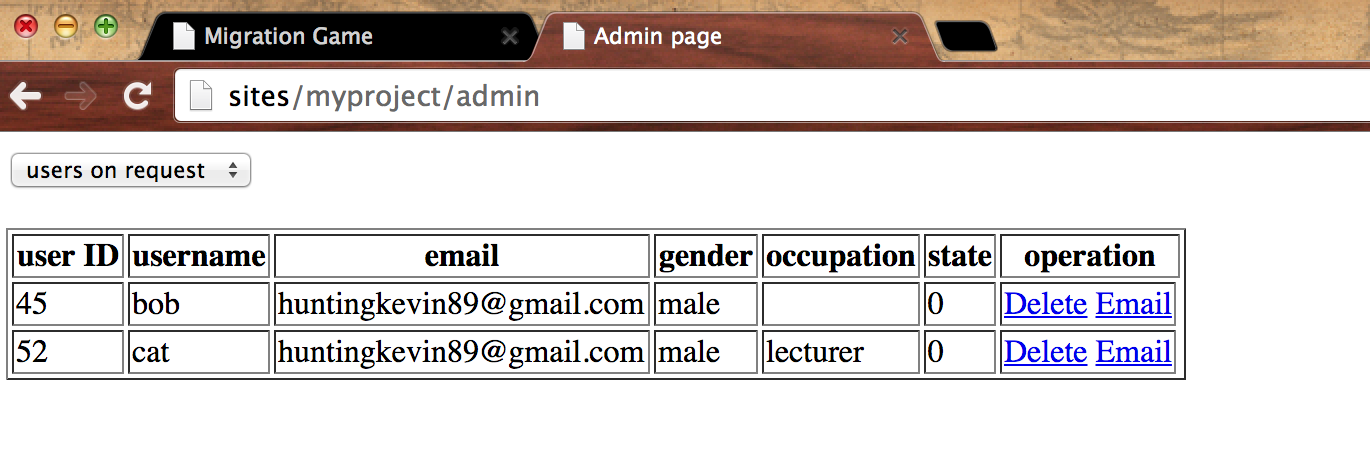
\includegraphics[width=14cm]{admin.png}
  \caption{Administrator page}
  \label{Figure:admin}
\end{figure}

\section{Game Page}
Game page is definitely the core of the application. Final interface is illustrated in the appendix. As the design described in Chapter 3, the project has two main classes to build the game page. The PHP file "login .php" is to test whether the user is in the database and if it matches, HTML page will be loaded. For log on component, it is accomplished as Listing 4.4 shows. If the post command is not "post", it will exit alerting that it is an invalid access in order to make sure there is only one entrance to enter the game. People cannot play the game by just using the url, but instead, entering through log on window is necessary. Otherwise a warning would be shown. The page is programmed by "echo" and using html syntax. 
\begin{lstlisting}[caption=Code of log on component]
if(!isset($_POST['submit'])){
        exit('Invalid access!');
    }
    
    $username = $_POST['username'];
    $password = md5($_POST['password']);

    //connect to database
    include('conn.php');
    // check if user exists
    $sql="select uid from user where username='$username' and password='$password'";

\end{lstlisting}

To make the page clearer, the html page is split into three divisions - \textit{information, chessboard and operation}. Information block contains a begin button which should be clicked to start the game and a textarea below to display on which step the user is and provide guidance. The prisoner's dilemma matrix which is created using a $\langle table \rangle$ element and icon representation are displayed at the end of this division. 

The chessboard division is a table with double borders so that it can be more stereoscopic. What is more, in order to set the cross of two lines as a point that can be placed other elements  like black and white chesses, this web application creates $\langle i \rangle$ elements whose class name are called "iBox" and configures in the stylesheet to fix every position of $\langle i \rangle$ components. To generate them, the project utilises some basic interface classes such as "addClass" and "createElement" in JavaScript. In Listing 4.5, an $\langle i \rangle$ element is created and set the style left and top value as i and j increase, then it is given an id. Additionally, building a map should have an array to know which point is empty or occupied. In this development, 50 random indexes are assigned as defectors or cooperators and the rest are undefined which means they are vacant. If one point is occupied, it will have a question mark covered on it. Eventually, the initial location of the player is fixed, but neighbours are random as well.

\begin{lstlisting}[caption=Part of code to create a map]
iBox=document.createElement("div");
	iBox.className="iBox";
	for(var i=0;i<10;i++)
		for(var j=0;j<10;j++){
			var iObj=document.createElement("i");
			iObj.appendChild(document.createTextNode(i*10+j));
			iObj.style.left=j*41+1+"px";
			iObj.style.top=i*41+1+"px";
			iObj.id=i*10+j;
			iObj.className="piece";
			iBox.appendChild(iObj);
			iArray.push(iObj);
	}

\end{lstlisting}


To make the page as simple as possible, the operation division is implemented as a three-layer wrapper which can be seen in Listing 4.6. In $\langle form \rangle$, because every bottom element has a style setting that padding-bottom is 330 pixels, only one $\langle div \rangle$ can be seen one time. The "step1" has a button that links to "step2" so that when the button is pressed, "step1" will disappear and just "step2" is visible. This simplicity can be concise and friendly enough for users to manipulate during the game.
\begin{lstlisting}[caption=Part of the code to wrap elements]
<div id="form_main_wrapper">
                <div id="form_main">
                    <div id="form_content">
                    	<div id="step1" style="padding-bottom: 330px">...</div>
                    	<div id="step2">...</div>
                    	...

\end{lstlisting}

The second problem is how to handle every click event and make the game procedure go fluently. For the click on the map, jQuery is used to listen to every element. As can be seen in Listing 4.7, when element of "i.piece" is clicked, the function will be activated. If tMove which counts the step for a user to move is less than one, the class name will be changed to "piece man" which is defined in the stylesheet to add the man picture on the point and remove the picture of previous location by deleting "man" from the class name. Furthermore, it calculates the coordinate of the clicking position and save it in a invisible element. It is similar for the method to explore three locations except one thing. Exploring needs to calculate the payoff of the point at the same time, so a local variable is created to remember the total bonus computed according to the prisoner's dilemma matrix. Then the value is saved in a hidden element.

\begin{lstlisting}[caption=Part of the code to move the player]
function movePlayer(){
	$("i.piece").click(function(){
		if(tMove<1){
			tMove++;
			if(iPoint[this.id]==undefined){
				var pieceObj=document.getElementById(this.id);
				var manObj=document.getElementsByClassName("piece man")[0];
				manObj.className="piece";
				pieceObj.className="piece man";
				var x=this.id%10;
				var y=parseInt(this.id/10);
				pPosition=this.id;
				pxy="("+x+","+y+")";
			}
                    	...

\end{lstlisting}

Buttons in the operation division includes strategy choice of cooperation and defection. However, the most important clicking event of this segment is the "continue" button which connects to the next step to make the whole game run influently. It is achieved by the method \textit{"window.location.href"}.

The game page is finally implemented as \fref{Figure:game}. Information module is on the left and in the middle is the chessboard-like lattice. Users can operate from the operation module on the right of the window.
\begin{figure}[!htb]
  \centering
  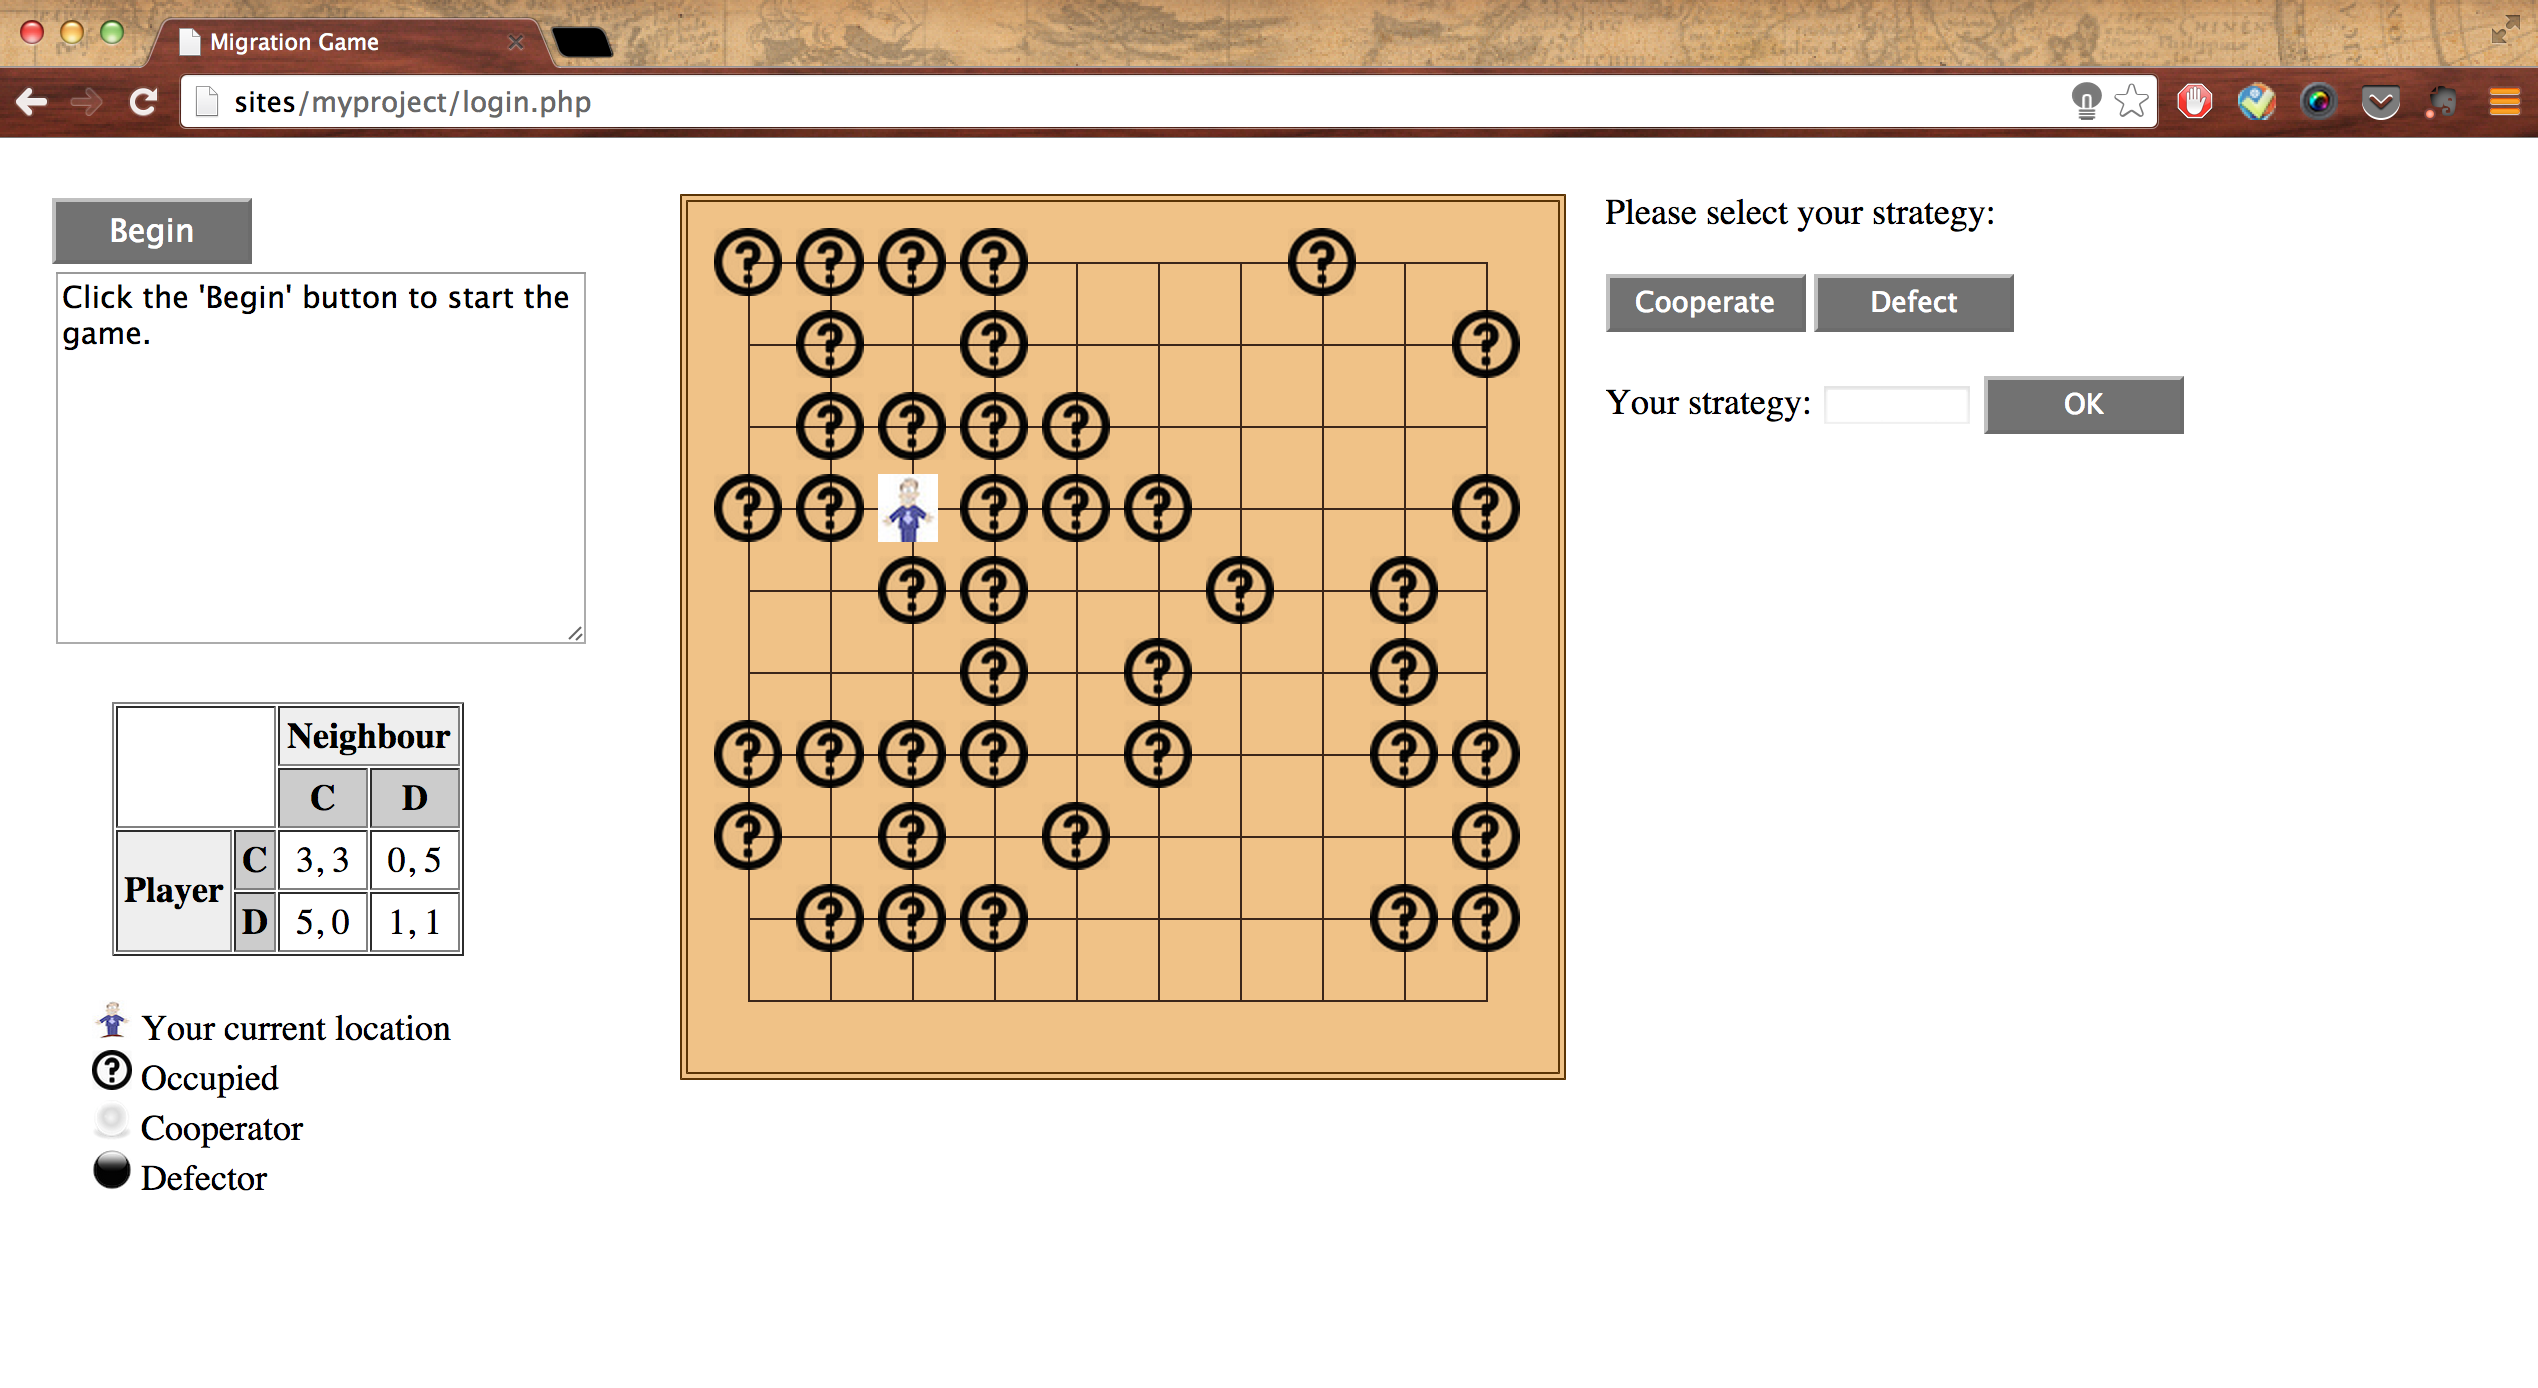
\includegraphics[width=14cm]{game.png}
  \caption{Game page}
  \label{Figure:game}
\end{figure}

Finally, when a game ends, results will be shown by getting data from database of the final record.

\section{Database Operation}
To provide operation of database, connection between front end and back end should be built at first which is written in PHP. To be specific, the project uses "mysql connect" function to create link and "mysql select db" to choose an exact database. In HTML, every component which needs to communicate with database would be programmed in a $\langle form \rangle$ element and deliver data by "post" method. When data is submitted, the page would direct to the corresponding php file and pass the data. Different SQL queries of select, update, insert and delete are used. Select query is for administrators' and users' name and password check, and once a requesting user is approved, updating sentence is run for saving password and change state value. Moreover, when a new user registers and a new game record is ready to save, data will be inserted. Deleting action is just for database management if a user is not agreed.

Many hidden elements are used in the game page as to temporarily save helpful data during the game. For instance, when a user clicks an empty point to explore, the coordinate and its payoff will be calculated and stored in an invisible component. When data is eventually submitted, all information in these elements will delivered at the same time.

Data lists stored in database consist of user, administrator and game record. Part of stored data is shown in \fref{Figure:record}.
\begin{figure}[!htb]
  \centering
  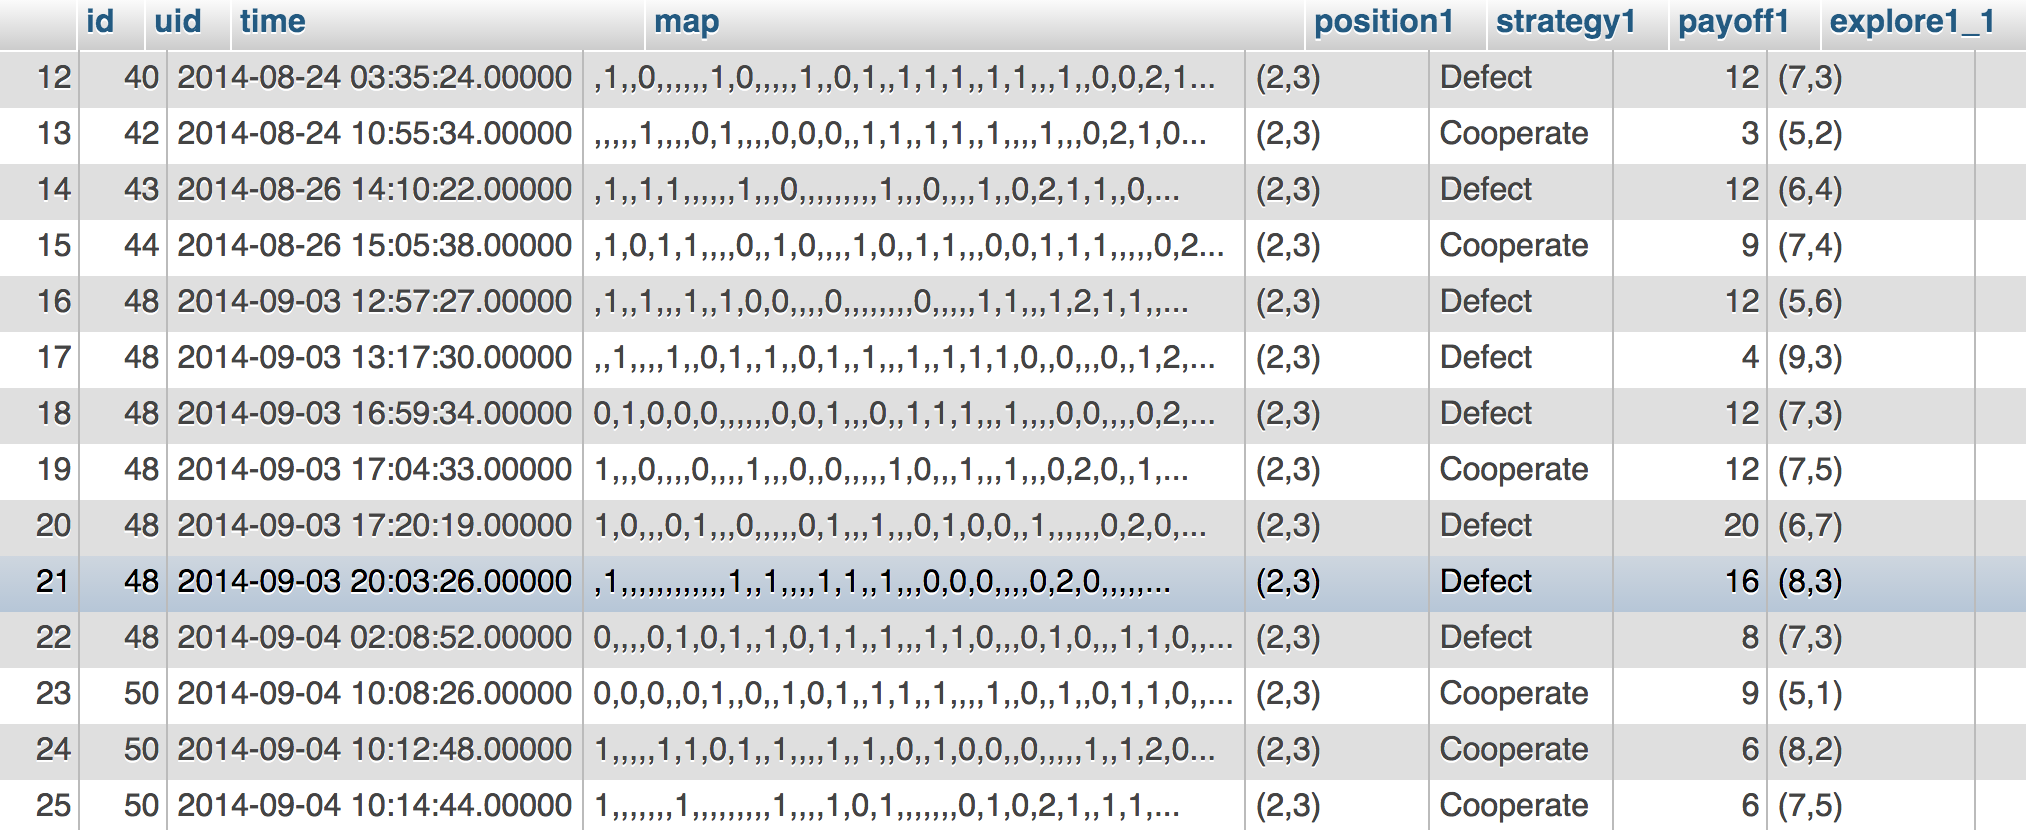
\includegraphics[width=14cm]{recordtable.png}
  \caption{Part of record table}
  \label{Figure:record}
\end{figure}

\chapter{Testing}
\section{Overall Testing}
At the end of development, testing is the most important procedure for the reason that it can discover problems and correct in time. Furthermore, users' feeling can be obtained first and that is helpful to improve the application to be more user-friendly. In this section, two aspects will be tested respectively.
\subsection{Compatibility}
There are all kinds of web browsers in market and users' preference cannot be predicted, thus compatibility of mainstream browsers is vital when functionality of the application is accomplished. Here, eight key browsers are chosen and tested, as can be seen in \tref{Table:compatibility}. The game can run on most browsers including Internet Explorer, Google Chrome, Firefox and Safari which should currently be the biggest four explorers. It can be smoothly running on all the up-to-date versions without any compatibility problems. However, when testing on Dooble, it is found that log on window could not normally show up and because of this, it is impossible to enter the game. The reason is probably this browser does not support JavaScript and PHP very well. Another similar issue happens on Netsurf which is an open source and light explorer which has its own layout engine. Opening the log-on page is successful but when trying to access the game, the lattice could not display whose reason may be deficiency of good compatibility with JavaScript. In addition, the application is tested on OmniWeb and it turns out no problem.

\begin{table}[!htb]
\centering
\begin{tabular}{|c|c|c|c|c|}
\hline
\textbf{Browser} & \specialcell{Dooble \\v1.48} & \specialcell{Google Chrome \\ v37.0 } & \specialcell{OmniWeb \\ v5.11} & \specialcell{Maxthon \\ v4.1.3} \\ \hline
\specialcell{\textbf{Instruction module} \\ \textbf{compatibility}} & \checkmark & \checkmark & \checkmark & \checkmark \\ \hline
\specialcell{\textbf{Log-on module} \\ \textbf{compatibility}}& \text{\sffamily X} & \checkmark & \checkmark & \checkmark \\ \hline
\specialcell{\textbf{Game module} \\ \textbf{compatibility}}& \text{\sffamily X} & \checkmark & \checkmark & \checkmark \\ \hline
\textbf{Browser} & \specialcell{Firefox \\ v32.0} & \specialcell{Netsurf \\ v2.9}  & \specialcell{Safari \\ v7.0.6}  & \specialcell{Internet \\ Explorer 11} \\ \hline
\specialcell{\textbf{Instruction module} \\ \textbf{compatibility}} & \checkmark & \checkmark & \checkmark & \checkmark \\ \hline
\specialcell{\textbf{Log-on module} \\ \textbf{compatibility}}& \checkmark & \checkmark & \checkmark & \checkmark \\ \hline
\specialcell{\textbf{Game module} \\ \textbf{compatibility}}& \checkmark & \text{\sffamily X} & \checkmark & \checkmark \\ \hline

\end{tabular}
\caption{Compatibility with main web browsers}
\label{Table:compatibility}
\end{table}

Therefore, the application is compatible with main internet browsers, although it cannot run well on some browsers which have their own engine and it may be the cause of the issue.

\subsection{Usability}
Contrast colours are used in the application in order to make the page more clear to read. In addition, font-size is big to read and buttons are friendly to click with reasonable size and attractive colours. Moreover, game procedure is fluent although users should click a button every time a step is finished.

In terms of accessibility, it does not aim to accessibility use, so when it is tested according to Web Content Accessibility Guidelines (WCAG 2.0) which is developed by W3C and organisations around the world and aims to provide standard for web content accessibility, most of content are not satisfied. For example, not all functionality is available from a keyboard and content cannot be presented in different ways. Nevertheless, readability is achieved so that a few people with disabilities can participate in this game.
\section{Evaluation}
As discussed above, the project is to create an application about migration in prisoner's dilemma game. 
\subsection{Disadvantages and Issues} \label{Subsubsection: dis}
\begin{enumerate}
\item Do not solve the calculating error when line breaks. In this application, an array is used to remember strategies of every person and empty locations on the map - "0" is cooperation, "1" is defection, "2" is the location of the play and "undefined" means empty. When calculating payoff of a specific point, it just utilises the strategy array because every index represents a definite point and if a point is known, its neighbours to the top, right, bottom and left can compute. However, when a clicked point is on the edge of the chessboard and coincidently on the first point of next line whose index is actually next to the one clicked in the strategy array. Therefore, when calculating payoff, mistakes may happen. For correcting it, "if" statement should be added when the user clicks points on the edge.
\item Not support configuration of the game. At the moment, payoff matrix is fixed and set by the programmer, so every player plays the same game. Nevertheless, the application should be more flexible that it can be configured by administrators. For example, the matrix can be modified to snowdrift game and observe what human strategies are to compare with prisoner's dilemma.
\item Registering detail is not sufficient. Administrators need to control or monitor the game and users, so there should be enough information for them to consider if the user can participate the game. At the moment, information a user must enter is just name, email, gender and occupation which may be insufficient for the manager. Moreover, later analysis can be categorised based on this information which can be very meaningful.
\item Neighbours are all static, initialising at the beginning. Information on the map including the player's initial location and all strategies of occupied positions are set when the game starts and never change during the game. This means computer players are not intelligent to apply some classic solution like "Tit-for-Tat" or "win-stay, lose shift". This may decrease meaning of collecting the data to study human cooperative motivation.
\end{enumerate}

\subsection{Advantages and Benefits}
\begin{enumerate}
\item Secure. This project applies an encryption algorithm to encryption user's password when it is stored into database. By doing this, password is secure when transmitting and also, even the administrator is not able to know the password from the table in the database. In addition, the project allows a manager to approve or reject a user to join which means not only not all people who want to join can participate as they want but also all users are verified and they are monitored in the game. Finally, the proof of security is that the only way to join the game is logging on. If a person tries to directly enter by URL, it will return error. 
\item Concise user interface. User interface of the game page is clear to divide into three main components and users can easily access through logging on. Every time on the operation module, there are only buttons regarding to the current step. This may help users focus on what they need to do and make them feel less lost and more user-friendly.
\end{enumerate}

%% ----------------------------------------------------------------
%% Conclusions.tex
%% ---------------------------------------------------------------- 


\chapter{Conclusion and Future Work} \label{Chapter: Conclusion}
In this dissertation, design and implementation of a Web application on prisoner's dilemma games where migration is possible are introduced. It is for users to have fun, simulating migration in reality when some neighbours have cooperation or defection strategies. In this game, users should try their best to acquire more payoff, by making decisions of strategies to play against their nearest individuals and of a new location they want to move to for four rounds. It may be not enough to collect usefully researched information, but it is just a beginning. In the future, it can be extended. In addition, it can help researchers in the future to find out what strategies of human when they migrate. Data of the game is stored in the database, including strategy of every round and its corresponding bonus which can record variety of a player's decisions.

In the future, work can continue as the following directions:
\begin{itemize}
\item Mistakes of payoff calculation which is discussed in \cref{Subsubsection: dis} should be debug and corrected. One solution may be adding a restricted condition before the clicking event runs. It could be checking if the id value of choosing site is 9, 18, 27,\dots , which are the edge of the right border. If so, the right neighbour will be ignored. Similarly, if the id value equals to 10, 20, 30, \dots , it should ignore the left-hand-side neighbour.
\item Specific configuration can be modified by the administrator. At the moment, payoff matrix is satisfied with prisoner's dilemma and it cannot be changed unless directly changing the source code. This, however, is not realistic in most cases. Therefore, another component should be added into administrator's page which can show the specific features of the game, such as fitness table, size of the map and so on and managers can modify them. Additionally, more personal detail may be required in the future which can give the administrator more reference of the user.
\item Computer players should be more intelligent. The computer players are all set at the beginning of the game and fixed during the whole game. After this project, intelligence of the computer should be improved, maybe using some solutions like "tit-for-tat" and "win-stay, lose-shift". It can increase the game's fun.
\end{itemize}











%\appendix
%%% ----------------------------------------------------------------
%% AppendixA.tex
%% ---------------------------------------------------------------- 


\chapter{Stuff} \label{Chapter:Stuff}
The following gets in the way of the text....

\backmatter
\bibliographystyle{apalike}
\bibliography{ECS}
\end{document}
%% ----------------------------------------------------------------
